% ============================================================================
%  Mémoire de Master — Ingénierie des Systèmes et Réseaux
%  Conception et mise en œuvre d'une infrastructure CI/CD
%  pour le firmware d'un produit de comptage d'énergie
%
%  Compilation :  make        (via Docker, voir Makefile)
%                 latexmk -pdf main.tex   (si TeX Live installé localement)
% ============================================================================
% Classe book : nécessaire pour \frontmatter / \mainmatter / \backmatter.
\documentclass[a4paper,11pt,twoside,openright]{book}

% ============================================================================
%  preamble.tex — Configuration du document
% ============================================================================

% ---------------------------------------------------------------------------
%  Langue et encodage
% ---------------------------------------------------------------------------
\usepackage[T1]{fontenc}
\usepackage[utf8]{inputenc}
\usepackage{lmodern}
\usepackage[french]{babel}
\usepackage[autostyle,french=guillemets]{csquotes}
\frenchsetup{SmallCapsFigTabCaptions=false}

% ---------------------------------------------------------------------------
%  Mise en page
% ---------------------------------------------------------------------------
\usepackage[a4paper,inner=3cm,outer=2.5cm,top=2.5cm,bottom=2.5cm]{geometry}
\usepackage{setspace}
\onehalfspacing
\usepackage{emptypage}
\usepackage{fancyhdr}
\pagestyle{fancy}
\fancyhf{}
\fancyhead[LE,RO]{\thepage}
\fancyhead[RE]{\nouppercase{\leftmark}}
\fancyhead[LO]{\nouppercase{\rightmark}}
\renewcommand{\headrulewidth}{0.4pt}
\fancypagestyle{plain}{%
  \fancyhf{}%
  \fancyfoot[C]{\thepage}%
  \renewcommand{\headrulewidth}{0pt}%
}

% ---------------------------------------------------------------------------
%  Graphiques, tableaux, flottants
% ---------------------------------------------------------------------------
\usepackage{graphicx}
\graphicspath{{figures/}}
\usepackage{amssymb}   % \checkmark
\usepackage{booktabs}
\usepackage{tabularx}
\usepackage{longtable}
\usepackage{multirow}
\usepackage{float}
\usepackage[font=small,labelfont=bf]{caption}
\usepackage{subcaption}
\usepackage{xcolor}
\usepackage{enumitem}

% ---------------------------------------------------------------------------
%  Listings (extraits YAML, Bash, Dockerfile, HCL)
% ---------------------------------------------------------------------------
\usepackage{listings}

\definecolor{codebg}{RGB}{248,248,248}
\definecolor{codeframe}{RGB}{210,210,210}
\definecolor{codekw}{RGB}{0,86,160}
\definecolor{codestr}{RGB}{163,21,21}
\definecolor{codecmt}{RGB}{96,139,78}

\lstdefinestyle{sestyle}{
  backgroundcolor=\color{codebg},
  basicstyle=\ttfamily\footnotesize,
  keywordstyle=\color{codekw}\bfseries,
  stringstyle=\color{codestr},
  commentstyle=\color{codecmt}\itshape,
  numbers=left,
  numberstyle=\tiny\color{gray},
  numbersep=8pt,
  frame=single,
  rulecolor=\color{codeframe},
  breaklines=true,
  breakatwhitespace=true,
  showstringspaces=false,
  tabsize=2,
  captionpos=b,
  literate=%
    {é}{{\'e}}1 {è}{{\`e}}1 {ê}{{\^e}}1 {à}{{\`a}}1
    {ù}{{\`u}}1 {ç}{{\c c}}1 {ô}{{\^o}}1 {î}{{\^\i}}1
}
\lstset{style=sestyle}

% Langages non connus de listings
\lstdefinelanguage{yaml}{
  keywords={true,false,null,on,off,needs,runs-on,uses,with,env,jobs,steps,name,
            strategy,matrix,inputs,secrets,if,run,outputs,permissions},
  sensitive=false,
  comment=[l]{\#},
  morestring=[b]",
  morestring=[b]'
}
\lstdefinelanguage{docker}{
  keywords={FROM,RUN,COPY,ADD,ARG,ENV,WORKDIR,USER,ENTRYPOINT,CMD,LABEL,SHELL,AS},
  sensitive=true,
  comment=[l]{\#},
  morestring=[b]"
}
\lstdefinelanguage{hcl}{
  keywords={resource,module,variable,output,provider,locals,data,terraform,for_each,source},
  sensitive=true,
  comment=[l]{\#},
  morestring=[b]"
}

% ---------------------------------------------------------------------------
%  Bibliographie
% ---------------------------------------------------------------------------
\usepackage[backend=biber,style=numeric,sorting=nyt,maxbibnames=99,giveninits=true]{biblatex}
\addbibresource{biblio.bib}

% ---------------------------------------------------------------------------
%  Acronymes / glossaire
% ---------------------------------------------------------------------------
\usepackage[acronym,nonumberlist,nopostdot,nomain]{glossaries}
\makeglossaries

% ---------------------------------------------------------------------------
%  Notes de rédaction  (mettre \setboolean{draftmode}{true} pour la version finale)
% ---------------------------------------------------------------------------
\usepackage{ifthen}
\newboolean{draftmode}
\setboolean{draftmode}{true}

\usepackage[colorinlistoftodos,prependcaption,textsize=footnotesize,french]{todonotes}
\ifthenelse{\boolean{draftmode}}{}{\presetkeys{todonotes}{disable}{}}

% Raccourcis de rédaction
\newcommand{\aecrire}[1]{\todo[inline,color=orange!25]{À RÉDIGER : #1}}
\newcommand{\chiffre}[1]{\todo[inline,color=red!25]{CHIFFRE À MESURER : #1}\textbf{40 Milliards d'euros}}
\newcommand{\verifier}[1]{\todo[color=blue!25]{VÉRIFIER : #1}}

% ---------------------------------------------------------------------------
%  ANONYMISATION
%  Tant que l'autorisation de publication n'est pas obtenue, basculer
%  \setboolean{confidentiel}{true} : tous les noms sensibles sont remplacés.
% ---------------------------------------------------------------------------
\newboolean{confidentiel}
\setboolean{confidentiel}{false}

\ifthenelse{\boolean{confidentiel}}{%
  \newcommand{\Entreprise}{l'entreprise}
  \newcommand{\Produit}{le produit P}
  \newcommand{\ProduitCourt}{P}
  \newcommand{\Firmware}{le firmware applicatif}
  \newcommand{\Carte}{la carte cible}
  \newcommand{\SrvCoverity}{\texttt{<serveur-sast-interne>}}
  \newcommand{\SrvBDBA}{\texttt{<serveur-sca-interne>}}
  \newcommand{\SrvArtifacts}{\texttt{<artifactory-interne>}}
  \newcommand{\SrvGit}{\texttt{<github-entreprise>}}
}{%
  \newcommand{\Entreprise}{Schneider Electric}
  \newcommand{\Produit}{le PM77xx}
  \newcommand{\ProduitCourt}{PM77xx}
  \newcommand{\Firmware}{SDP}
  \newcommand{\Carte}{bru99379-kp0}
  \newcommand{\SrvCoverity}{\texttt{coverity-embu.se.com}}
  \newcommand{\SrvBDBA}{\texttt{bdba.schneider-electric.com}}
  \newcommand{\SrvArtifacts}{\texttt{global-artifacts.se.com}}
  \newcommand{\SrvGit}{\texttt{github.schneider-electric.com}}
}

% ---------------------------------------------------------------------------
%  Hyperliens (à charger en dernier ou presque)
% ---------------------------------------------------------------------------
\usepackage[hidelinks,breaklinks=true]{hyperref}
\hypersetup{
  pdftitle={Conception et mise en oeuvre d'une infrastructure CI/CD pour le firmware d'un produit de comptage d'energie},
  pdfsubject={Memoire de Master Ingenierie des Systemes et Reseaux},
  pdfkeywords={CI/CD, DevOps, systemes embarques, Yocto, GitHub Actions, analyse statique, SBOM, Infrastructure as Code}
}
\usepackage[french]{cleveref}

% ============================================================================
%  config/acronymes.tex — Liste des acronymes
% ============================================================================

\newacronym{ci}{CI}{Continuous Integration (intégration continue)}
\newacronym{cd}{CD}{Continuous Delivery / Deployment (livraison / déploiement continu)}
\newacronym{cicd}{CI/CD}{Intégration et livraison continues}
\newacronym{sast}{SAST}{Static Application Security Testing}
\newacronym{dast}{DAST}{Dynamic Application Security Testing}
\newacronym{sca}{SCA}{Software Composition Analysis}
\newacronym{sbom}{SBOM}{Software Bill of Materials}
\newacronym{bdba}{BDBA}{Black Duck Binary Analysis}
\newacronym{iac}{IaC}{Infrastructure as Code}
\newacronym{raas}{RaaS}{Runner Orchestrator as a Service}
\newacronym{dora}{DORA}{DevOps Research and Assessment}
\newacronym{mttr}{MTTR}{Mean Time To Restore}
\newacronym{bsp}{BSP}{Board Support Package}
\newacronym{sdk}{SDK}{Software Development Kit}
\newacronym{soc}{SoC}{System on Chip}
\newacronym{som}{SOM}{System on Module}
\newacronym{tpm}{TPM}{Trusted Platform Module}
\newacronym{sdp}{SDP}{Schneider Device Platform}
\newacronym{csb}{CSB}{Cyber Security Brick}
\newacronym{nbi}{NBI}{North Bound Interface}
\newacronym{edm}{EDM}{Equipment Data Model}
\newacronym{api}{API}{Application Programming Interface}
\newacronym{rest}{REST}{Representational State Transfer}
\newacronym{cve}{CVE}{Common Vulnerabilities and Exposures}
\newacronym{cvss}{CVSS}{Common Vulnerability Scoring System}
\newacronym{cra}{CRA}{Cyber Resilience Act}
\newacronym{sdl}{SDL}{Secure Development Lifecycle}
\newacronym{vcs}{VCS}{Version Control System}
\newacronym{pr}{PR}{Pull Request}
\newacronym{ut}{UT}{Unit Test (test unitaire)}
\newacronym{qa}{QA}{Quality Assurance}
\newacronym{iam}{IAM}{Identity and Access Management}
\newacronym{aws}{AWS}{Amazon Web Services}
\newacronym{vm}{VM}{Machine virtuelle}
\newacronym{tsdb}{TSDB}{Time Series Database}
\newacronym{yaml}{YAML}{YAML Ain't Markup Language}
\newacronym{json}{JSON}{JavaScript Object Notation}
\newacronym{ssh}{SSH}{Secure Shell}
\newacronym{pat}{PAT}{Personal Access Token}
\newacronym{lts}{LTS}{Long Term Support}


\begin{document}

% --------------------------------------------------------------- Pages liminaires
\frontmatter
\pagenumbering{roman}

% ============================================================================
%  frontmatter/page-de-garde.tex
%  TODO : remplacer les champs entre crochets par les informations réelles
%         (établissement, logo, nom des encadrants, jury, promotion).
% ============================================================================
\begin{titlepage}
\centering
\thispagestyle{empty}

% --- Logos : déposer les fichiers dans figures/ puis décommenter -------------
% \begin{minipage}{0.45\textwidth}\raggedright
%   \includegraphics[height=2cm]{logo-universite}
% \end{minipage}\hfill
% \begin{minipage}{0.45\textwidth}\raggedleft
%   \includegraphics[height=2cm]{logo-entreprise}
% \end{minipage}

\vspace{1.5cm}

{\large \textsc{[Nom de l'établissement]}}\\[0.3cm]
{\large [Faculté / Département]}\\[1.5cm]

{\large \textbf{MÉMOIRE DE FIN D'ÉTUDES}}\\[0.3cm]
{\normalsize présenté en vue de l'obtention du diplôme de}\\[0.3cm]
{\large \textbf{Master en Ingénierie des Systèmes et Réseaux}}\\[2cm]

\rule{\textwidth}{0.8pt}\\[0.6cm]
{\LARGE \bfseries Conception et mise en œuvre d'une infrastructure
d'intégration et de livraison continues pour le firmware d'un produit
industriel de comptage d'énergie\par}
\vspace{0.6cm}
\rule{\textwidth}{0.8pt}\\[2cm]

\begin{minipage}{0.45\textwidth}\raggedright
  \textbf{Présenté par :}\\[0.2cm]
  [Prénom NOM]
\end{minipage}\hfill
\begin{minipage}{0.45\textwidth}\raggedleft
  \textbf{Encadrant académique :}\\[0.2cm]
  [Prénom NOM]\\[0.5cm]
  \textbf{Encadrant entreprise :}\\[0.2cm]
  [Prénom NOM], \Entreprise
\end{minipage}

\vfill

{\normalsize Travail réalisé au sein de \Entreprise\\[0.3cm]
Année universitaire [20XX--20XX]}\\[0.5cm]
{\normalsize Soutenu le [JJ mois AAAA]}

\end{titlepage}
\cleardoublepage

% ============================================================================
%  frontmatter/confidentialite.tex
%  À conserver tant que l'autorisation de publication n'a pas été obtenue.
%  Si le mémoire est rendu public, supprimer l'inclusion depuis main.tex.
% ============================================================================
\thispagestyle{empty}
\vspace*{4cm}
\begin{center}
{\Large \bfseries Clause de confidentialité}
\end{center}
\vspace{1cm}

\noindent
Le présent mémoire a été réalisé dans le cadre d'un projet industriel mené au
sein de \Entreprise. Il décrit une infrastructure interne d'intégration et de
livraison continues ainsi que les outils et processus associés.

\medskip
\noindent
Certaines informations (dénominations commerciales, identifiants de projets, valeurs de mesures) ont été anonymisées ou
omises afin de préserver la confidentialité des données de l'entreprise. Les
éléments techniques présentés le sont à des fins exclusivement pédagogiques et
d'évaluation académique.

\medskip
\noindent
La diffusion de ce document est restreinte aux membres du jury et aux
personnels de l'établissement habilités, sauf autorisation écrite contraire de
\Entreprise.

\vfill
\clearpage

% ============================================================================
%  frontmatter/remerciements.tex
% ============================================================================
\chapter*{Remerciements}
\addcontentsline{toc}{chapter}{Remerciements}
\markboth{Remerciements}{Remerciements}

\aecrire{Une page maximum. Ordre habituel : encadrant entreprise, équipe
technique / DevOps, encadrant académique, établissement, proches. Rester
sobre et nommer les personnes.}

Je tiens à remercier [Prénom NOM], mon encadrant au sein de \Entreprise, pour
[la confiance accordée / l'autonomie laissée sur le projet / ses relectures].

\medskip
Mes remerciements vont également à l'ensemble de l'équipe [nom de l'équipe],
qui [\ldots].

\medskip
Je remercie enfin [Prénom NOM], mon encadrant académique, ainsi que les membres
du jury qui ont accepté d'évaluer ce travail.

\cleardoublepage

% ============================================================================
%  frontmatter/resume.tex — Résumé FR + Abstract EN
%  À rédiger EN DERNIER (J12), une fois les résultats connus.
%  Cible : 200 à 250 mots chacun. Structure IMRaD condensée :
%  contexte -> problème -> méthode -> résultats chiffrés -> portée.
% ============================================================================
\chapter*{Résumé}
\addcontentsline{toc}{chapter}{Résumé}
\markboth{Résumé}{Résumé}

Le développement du firmware des produits industriels embarqués se heurte à des
cycles d'intégration longs, à des environnements de compilation hétérogènes et
à des exigences de cybersécurité croissantes. Ce mémoire présente la conception et la mise
en œuvre d'une infrastructure d'intégration
et de livraison continues pour le firmware du module de communication d'un
compteur d'énergie (\emph{Power Meter}) développé chez \Entreprise, module
chargé d'intégrer les protocoles Modbus, Ethernet, BACnet et une API REST.

Le travail ne part pas d'une feuille blanche : il reprend une chaîne GitHub
Actions existante, en analyse les limites, formalise des exigences avec
l'équipe, puis la fait évoluer. Les évolutions portent sur une image de
compilation unique intégrant le kit de développement de la cible, une matrice
de construction native et croisée, la mesure de couverture, les tests
d'intégration, l'analyse de composition binaire, la publication des artefacts
et la collecte d'indicateurs vers VictoriaMetrics et Grafana.

L'évaluation porte sur 164 exécutions sur cinq semaines. La chaîne applicative
rend un résultat complet en 21,8 minutes en médiane, la parallélisation de la
matrice réduisant sa durée d'environ un tiers. La chaîne restitue à chaque
exécution la couverture (32,3~\% des lignes), les défauts d'analyse statique et
l'inventaire des composants tiers avec leurs vulnérabilités. La distribution
Linux reste reconstruite sans cache en 68,2 minutes, ce qui fait du cache partagé
la principale perspective.

\vspace{1cm}
\noindent\textbf{Mots-clés :} intégration continue, livraison continue, DevOps,
systèmes embarqués, Yocto, analyse statique, chaîne d'approvisionnement
logicielle, analyse de composition, observabilité.

\vfill

\section*{Abstract}
\markboth{Abstract}{Abstract}

The development of firmware for embedded industrial products is hindered by
long integration cycles, heterogeneous build environments, and growing
cybersecurity requirements. This
thesis presents the design and implementation of a continuous integration and
continuous delivery
infrastructure for the firmware of the communication module of an energy
meter (\emph{Power Meter}) developed at \Entreprise, a module responsible for
integrating the Modbus, Ethernet, BACnet, and REST API protocols.

Rather than starting from scratch, the work takes over an existing GitHub
Actions pipeline, analyses its limits, formalises requirements with the team
and evolves it: a single build image embedding the target SDK, a native and
cross-compilation build matrix, code coverage, integration tests, binary
composition analysis, artifact publication, and metrics collection into
VictoriaMetrics and Grafana.

The evaluation covers 164 runs over five weeks. The application pipeline
delivers a complete result in a median of 21.8 minutes, the parallel matrix
cutting its duration by about one third. Each run reports coverage (32.3\% of
lines), static analysis defects and the inventory of third-party components
with their vulnerabilities. The Linux distribution is still rebuilt without
cache in 68.2 minutes, which makes a shared build cache the main next step.

\vspace{1cm}
\noindent\textbf{Keywords:} continuous integration, continuous delivery, DevOps,
embedded systems, Yocto, static analysis, software supply chain,
software composition analysis, observability.

\clearpage


\clearpage
\tableofcontents
\clearpage
\listoffigures
\clearpage
\listoftables
\clearpage
\printglossary[type=\acronymtype,title={Liste des acronymes}]

\ifthenelse{\boolean{draftmode}}{\cleardoublepage\listoftodos[Travail restant]}{}

% --------------------------------------------------------------- Corps du mémoire
\mainmatter
\pagenumbering{arabic}
\setcounter{page}{1}

% ============================================================================
%  Chapitre 1 — Introduction
%  Cible : 4 à 5 pages. À RÉDIGER EN DERNIER (J12), après le chapitre 6.
% ============================================================================
\chapter{Introduction}
\label{chap:introduction}

\section{Contexte général}
\label{sec:intro-contexte}

\aecrire{4 à 6 paragraphes. Entonnoir : (1) électrification et numérisation des
réseaux électriques, place du comptage d'énergie communicant ; (2) le produit
n'est plus un équipement figé mais une plateforme logicielle mise à jour sur
le terrain ; (3) conséquence : la qualité et la sécurité du logiciel embarqué
deviennent un enjeu produit, pas un enjeu d'atelier ; (4) l'industrialisation
de la chaîne de production logicielle (CI/CD) devient donc un sujet
d'ingénierie à part entière.}

\section{Problématique}
\label{sec:intro-problematique}

Le développement du firmware d'un produit industriel embarqué cumule des
contraintes que l'on rencontre rarement simultanément dans le développement
logiciel classique :

\begin{itemize}[nosep]
  \item des temps de construction très longs, la génération d'une distribution
        Linux embarquée complète se comptant en heures et non en minutes ;
  \item un environnement de compilation complexe et fragile, associant chaînes
        de compilation croisée, bibliothèques système et outils propriétaires ;
  \item des exigences réglementaires et normatives de cybersécurité
        (IEC~62443-4-1, règlement (UE) 2024/2847 dit \emph{Cyber Resilience
        Act}) imposant la traçabilité des composants et la détection précoce
        des vulnérabilités ;
  \item une exécution des traitements sur une infrastructure mutualisée et
        éphémère, où aucun état ne persiste d'une exécution à l'autre.
\end{itemize}

\medskip
\noindent
Ces contraintes conduisent à la question de recherche suivante :

\begin{quote}
\itshape
Comment concevoir et mettre en œuvre une chaîne d'intégration et de livraison
continues reproductible, sécurisée et mesurable pour le firmware d'un produit
industriel embarqué, sous contraintes de temps de construction longs,
d'exigences normatives de cybersécurité et d'infrastructure d'exécution
éphémère ?
\end{quote}

\noindent
Cette question se décline en quatre sous-questions traitées respectivement dans
les sections~\ref{sec:impl-conteneur} à~\ref{sec:impl-observabilite} :

\begin{description}[style=nextline,leftmargin=1.5cm]
  \item[QR1 — Reproductibilité] Comment garantir qu'une même révision du code
        source produise un artefact identique, indépendamment de la machine et
        de la date d'exécution ?
  \item[QR2 — Sécurité] Comment intégrer l'analyse statique du code et
        l'analyse de composition logicielle dans le cycle de développement sans
        dégrader la vélocité des équipes de développement ?
  \item[QR3 — Mesurabilité] Quels indicateurs instrumenter pour piloter la
        qualité de la chaîne, et comment les collecter automatiquement ?
  \item[QR4 — Passage à l'échelle] Comment dimensionner et administrer
        l'infrastructure d'exécution de manière automatisée et maîtrisée en
        coût ?
\end{description}

\section{Objectifs et périmètre}
\label{sec:intro-perimetre}

\aecrire{Formuler 4 à 5 objectifs opérationnels mesurables, puis délimiter
explicitement ce qui est hors périmètre.}

Le périmètre de ce travail est la \emph{chaîne de production} du firmware, et
non le firmware lui-même. Sont explicitement exclus : la conception
fonctionnelle de l'application embarquée, le déploiement des mises à jour sur
le parc installé, ainsi que la conception matérielle du produit au-delà des
contraintes qu'elle impose à la compilation.

\section{Contributions}
\label{sec:intro-contributions}

Les contributions de ce travail sont les suivantes :

\begin{enumerate}[nosep]
  \item la conteneurisation de l'environnement de compilation applicatif, avec
        épinglage des versions de l'ensemble de la chaîne d'outils
        (chapitre~\ref{chap:mise-en-oeuvre}, section~\ref{sec:impl-conteneur}) ;
  \item la conception de deux chaînes d'intégration distinctes et
        complémentaires, l'une pour la couche applicative et l'autre pour la
        distribution Linux embarquée (sections~\ref{sec:impl-pipeline-app}
        et~\ref{sec:impl-pipeline-yocto}) ;
  \item l'intégration automatisée de l'analyse statique et de l'analyse de
        composition logicielle avec restitution des résultats au développeur
        (section~\ref{sec:impl-securite}) ;
  \item l'automatisation de l'infrastructure d'exécution par
        \emph{infrastructure as code} (section~\ref{sec:impl-runners}) ;
  \item la mise en place d'une chaîne d'observabilité restituant l'évolution
        des indicateurs de qualité dans le temps
        (section~\ref{sec:impl-observabilite}) ;
  \item une évaluation quantitative de la chaîne obtenue
        (chapitre~\ref{chap:evaluation}).
\end{enumerate}

\section{Méthodologie}
\label{sec:intro-methodologie}

\aecrire{Assumer explicitement la posture : étude de cas industrielle unique,
de type recherche-action. Décrire le déroulement : analyse de l'existant,
recueil des exigences auprès des équipes, conception itérative, mise en
production incrémentale, mesure. Citer la littérature sur l'étude de cas en
génie logiciel (Runeson \& Höst) pour asseoir la démarche.}

\section{Organisation du mémoire}
\label{sec:intro-plan}

Le chapitre~\ref{chap:contexte} présente le contexte industriel, le produit et
l'état initial de la chaîne de développement. Le chapitre~\ref{chap:etat-art}
dresse l'état de l'art de l'intégration continue, de son application aux
systèmes embarqués et des pratiques de sécurisation de la chaîne
d'approvisionnement logicielle. Le chapitre~\ref{chap:besoins} formalise les
exigences et présente l'architecture retenue ainsi que la justification des
choix technologiques. Le chapitre~\ref{chap:mise-en-oeuvre} détaille la mise en
œuvre. Le chapitre~\ref{chap:evaluation} évalue quantitativement les résultats
obtenus et en discute les limites. Le chapitre~\ref{chap:conclusion} conclut et
ouvre sur les perspectives.

% ============================================================================
%  Chapitre 2 — Contexte industriel et analyse de l'existant
%  Cible : 8 à 10 pages. À rédiger J2-J3.
% ============================================================================
\chapter{Contexte industriel et analyse de l'existant}
\label{chap:contexte}

\section{L'entreprise et l'entité d'accueil}
\label{sec:ctx-entreprise}

\aecrire{1,5 page maximum. Ne pas faire une plaquette commerciale : le jury
attend le \emph{contexte organisationnel du projet}, pas le chiffre
d'affaires. Points à couvrir : activité de la division, positionnement du
produit dans la gamme, composition et localisation des équipes,
articulation entre équipe de développement firmware et équipe DevOps,
rattachement de l'auteur.}

\section{Le produit et son logiciel embarqué}
\label{sec:ctx-produit}

\subsection{Fonction du produit}
\aecrire{Rôle d'une centrale de mesure / compteur d'énergie communicant :
acquisition des grandeurs électriques, journalisation, exposition des données
aux systèmes de supervision.}

\subsection{Architecture matérielle}
La cible matérielle repose sur un \gls{soc} Texas~Instruments AM642 intégré sur
un \gls{som}, associé à une carte porteuse. La configuration de construction
désigne cette cible par la machine Yocto \texttt{\Carte}.

\aecrire{Décrire : cœurs Cortex-A53 (Linux) et cœurs Cortex-R5F (temps réel),
mémoire, stockage eMMC, présence d'un \gls{tpm}. Insister uniquement sur ce
qui \emph{contraint la chaîne de construction} : compilation croisée
aarch64, firmware R5F à générer avec une chaîne d'outils propriétaire,
signature et chaîne de confiance au démarrage.}

\subsection{Pile logicielle}
\label{ssec:ctx-pile-logicielle}

La pile logicielle se décompose en trois couches, chacune associée à un rythme
de construction et à des outils différents :

\begin{table}[H]
\centering
\caption{Décomposition de la pile logicielle embarquée}
\label{tab:ctx-pile}
\begin{tabularx}{\textwidth}{@{}l X l@{}}
\toprule
\textbf{Couche} & \textbf{Contenu} & \textbf{Construction} \\
\midrule
Distribution & Noyau Linux, \gls{bsp}, paquets système, image disque &
  Yocto / kas \\
Sécurité & Brique de cybersécurité transverse (\gls{csb}) & Meson \\
Application & Services métier \Firmware{} (gestion d'équipement, de défauts,
  interfaces nord) & CMake \\
\bottomrule
\end{tabularx}
\end{table}

\aecrire{Décrire brièvement les services applicatifs : gestion
administrative et système, gestion des équipements, gestion des défauts,
notifications, et les interfaces nord Modbus, BACnet et \gls{edm}. Mentionner
l'organisation en dépôts multiples avec sous-modules Git, car c'est une
contrainte forte pour la chaîne d'intégration.}

\section{Organisation des dépôts}
\label{sec:ctx-depots}

\aecrire{Expliquer la séparation en dépôts : configuration d'image,
couches BSP et distribution, application, tests d'automatisation, images de
construction, configuration des exécuteurs, supervision. Justifier pourquoi
cette séparation complique l'intégration (versions croisées, cohérence des
références, secrets d'accès inter-dépôts). Un tableau des dépôts est plus
lisible qu'un paragraphe.}

\begin{table}[H]
\centering
\caption{Dépôts intervenant dans la chaîne de construction}
\label{tab:ctx-depots}
\begin{tabularx}{\textwidth}{@{}>{\raggedright\arraybackslash}p{4cm} X l@{}}
\toprule
\textbf{Dépôt} & \textbf{Rôle} & \textbf{Branche} \\
\midrule
\texttt{ci} & Workflows et scripts d'intégration & \texttt{main} \\
\texttt{docker-image} & Image de l'environnement de compilation & \texttt{main} \\
\texttt{evo-image-config} & Configuration kas / Yocto de la distribution & \texttt{scarthgap} \\
\texttt{sdp} & Code applicatif et sous-modules & \texttt{develop} \\
\texttt{automation-tests} & Suites de tests d'intégration & \texttt{main} \\
\texttt{runner-config} & Infrastructure des exécuteurs & \texttt{Prod} \\
\texttt{monitoring-ci} & Exportateurs de métriques & \texttt{main} \\
\bottomrule
\end{tabularx}
\end{table}

\section{Analyse de l'existant}
\label{sec:ctx-existant}

\aecrire{C'est LA section qui justifie tout le mémoire. Sans un « avant »
décrit honnêtement, le chapitre~6 n'a pas de point de comparaison. Décrire
la situation initiale sans la caricaturer.}

\subsection{Pratiques de construction initiales}
\aecrire{Construction sur poste de développeur, environnements divergents
d'un poste à l'autre, dépendances installées manuellement, absence de
version de référence de la chaîne d'outils.}

\subsection{Pratiques de test et de qualité initiales}
\aecrire{Tests unitaires exécutés à la demande, absence de mesure de
couverture historisée, analyse statique lancée ponctuellement en fin de cycle,
analyse de composants réalisée manuellement avant les jalons.}

\subsection{Limites identifiées}
\label{ssec:ctx-limites}

\aecrire{Formuler chaque limite de façon à ce qu'elle soit reprise telle
quelle comme exigence au chapitre~4 et comme critère d'évaluation au
chapitre~6. Une limite = une exigence = une mesure. Conserver cette
traçabilité, le jury la cherchera.}

\begin{table}[H]
\centering
\caption{Limites de la situation initiale et exigences induites}
\label{tab:ctx-limites}
\begin{tabularx}{\textwidth}{@{}l X l@{}}
\toprule
\textbf{Réf.} & \textbf{Limite constatée} & \textbf{Exigence} \\
\midrule
L1 & Environnements de construction divergents entre développeurs & EF1 \\
L2 & Détection tardive des régressions & EF2 \\
L3 & Analyse statique non systématique & EF4 \\
L4 & Inventaire des composants tiers non tenu à jour & EF5 \\
L5 & Absence de mesure historisée de la qualité & EF6 \\
L6 & Administration manuelle des machines d'exécution & ENF3 \\
\bottomrule
\end{tabularx}
\end{table}

\section{Synthèse}
\label{sec:ctx-synthese}

\aecrire{Un paragraphe de transition vers le chapitre~3 : avant de concevoir,
examiner ce que la littérature et l'industrie proposent pour ces problèmes.}

% ============================================================================
%  Chapitre 3 — État de l'art
%  Cible : 12 à 15 pages. À rédiger J4-J5.
%
%  RÈGLE : chaque section se termine par un paragraphe « ce que l'on retient
%  pour ce travail ». Un état de l'art qui ne redescend pas sur le cas traité
%  est systématiquement sanctionné.
% ============================================================================
\chapter{État de l'art}
\label{chap:etat-art}

\section{Intégration et livraison continues}
\label{sec:art-cicd}

\subsection{Origines et définitions}
L'intégration continue est définie comme la pratique consistant à intégrer
fréquemment le travail de chaque développeur dans une ligne principale
partagée, chaque intégration étant validée par une construction et une
exécution automatisées des tests~\cite{fowler2006ci,duvall2007ci}. La livraison
continue étend ce principe en maintenant en permanence le logiciel dans un état
déployable~\cite{humble2010cd}.

\aecrire{Distinguer clairement intégration continue, livraison continue et
déploiement continu. Préciser laquelle de ces trois pratiques est visée dans ce
travail et pourquoi le déploiement continu n'est pas applicable à un produit
matériel certifié.}

\subsection{Bénéfices et coûts rapportés}
\aecrire{S'appuyer sur les études empiriques : Hilton et al. sur l'usage et le
coût de l'intégration continue~\cite{hilton2016usage}, Vasilescu et al. sur
les effets qualité et productivité~\cite{vasilescu2015quality}, Ståhl et Bosch
sur la variabilité des mises en œuvre industrielles~\cite{stahl2014modeling}.
Mentionner les coûts : maintenance de la chaîne, temps d'attente, tests
instables.}

\subsection{Revues systématiques}
La revue systématique de Shahin et al.~\cite{shahin2017continuous} recense les
approches, outils et difficultés associés à l'intégration, la livraison et le
déploiement continus, et identifie notamment la durée des constructions et la
complexité des environnements de test comme obstacles récurrents.

\subsection{Ce que l'on retient}
\aecrire{2 à 3 phrases reliant explicitement au cas traité.}

\section{Spécificités des systèmes embarqués}
\label{sec:art-embarque}

\aecrire{Cœur de l'originalité du sujet. Points à traiter : compilation
croisée, dépendance au matériel pour les tests, durée des constructions de
distributions complètes, cycles de certification, impossibilité de déployer en
continu. S'appuyer sur Mårtensson et al.~\cite{martensson2016embedded} et
Lwakatare et al.~\cite{lwakatare2019devops}.}

\subsection{Construction de distributions Linux embarquées}
\aecrire{Présenter Yocto/OpenEmbedded : notion de couche, de recette, de
machine, de distribution ; rôle du cache d'état partagé et du cache de
téléchargement dans la réduction du temps de construction. Présenter kas comme
outil de description déclarative de la configuration de construction. Citer la
documentation du projet Yocto~\cite{yoctoref}.}

\subsection{Ce que l'on retient}
\aecrire{Justifier la séparation en deux chaînes distinctes, applicative et
distribution, qui sera reprise au chapitre~4.}

\section{Reproductibilité de la construction}
\label{sec:art-reproductibilite}

La reproductibilité des constructions, c'est-à-dire la capacité à obtenir un
artefact binaire identique à partir d'une même révision du code source, est
présentée par Lamb et Zacchiroli comme un levier d'intégrité de la chaîne
d'approvisionnement logicielle~\cite{lamb2022reproducible}.

\aecrire{Articuler deux niveaux : (1) reproductibilité \emph{stricte} au sens
bit à bit, difficile à atteindre ; (2) reproductibilité \emph{de
l'environnement}, par conteneurisation et épinglage des versions, qui est
l'objectif réaliste retenu ici. Assumer ce choix explicitement, c'est un point
de discussion probable en soutenance.}

\section{Analyse statique de code}
\label{sec:art-sast}

\aecrire{Présenter le principe de l'analyse statique, puis les résultats
empiriques : Beller et al. sur l'état de l'analyse statique dans les projets
open source~\cite{beller2016analyzing}, Zampetti et al. sur l'intégration des
outils d'analyse statique dans les chaînes d'intégration
continue~\cite{zampetti2017static}. Traiter la question centrale des faux
positifs et de la stratégie de traitement de la dette initiale.}

\subsection{Politique de blocage}
\aecrire{Question de conception importante : faire échouer la construction
sur détection de défaut, ou seulement notifier ? Présenter les deux postures
et leurs conséquences sur l'adoption par les équipes. Ce point sera tranché
au chapitre~4 et discuté au chapitre~6.}

\section{Sécurité de la chaîne d'approvisionnement logicielle}
\label{sec:art-supply-chain}

\subsection{Menaces}
Ohm et al. proposent une taxonomie des attaques visant la chaîne
d'approvisionnement des logiciels libres~\cite{ohm2020backstabber}.

\subsection{Nomenclature logicielle}
La nomenclature logicielle (\gls{sbom}) recense les composants entrant dans la
composition d'un produit. Les éléments minimaux attendus ont été définis par la
NTIA~\cite{ntia2021sbom}, et le format SPDX a été normalisé sous la référence
ISO/IEC~5962~\cite{iso5962}.

\subsection{Analyse de composition logicielle}
\aecrire{Principe de l'analyse de composants binaires : identification des
composants embarqués dans un artefact compilé, corrélation avec les bases
\gls{cve}, scores \gls{cvss}. Expliquer pourquoi l'analyse binaire est plus
adaptée qu'une analyse des seuls fichiers de dépendances dans un contexte
Yocto.}

\section{Cadre normatif et réglementaire}
\label{sec:art-normes}

La norme IEC~62443-4-1~\cite{iec62443_4_1} définit les exigences de cycle de
développement sécurisé pour les produits d'automatisation industrielle. Le
règlement (UE) 2024/2847~\cite{cra2024} introduit des obligations de
cybersécurité pour les produits comportant des éléments numériques, dont la
tenue d'une nomenclature logicielle et le traitement des vulnérabilités
pendant la durée de support.

\aecrire{Établir explicitement la correspondance entre les pratiques mises en
œuvre au chapitre~5 et les exigences normatives. C'est un argument fort, et
c'est ce qui différencie ce mémoire d'un simple travail d'outillage.}

\aecrire{Compléter le tableau ci-dessous à partir du texte de la norme :
pratiques de gestion des défauts de sécurité, de vérification et de gestion des
composants tiers. Une ligne par exigence, avec renvoi vers la section du
chapitre~5 qui la couvre.}

\begin{table}[H]
\centering
\caption{Correspondance entre exigences normatives et pratiques mises en œuvre}
\label{tab:art-normes}
\begin{tabularx}{\textwidth}{@{}l X l@{}}
\toprule
\textbf{Exigence} & \textbf{Intitulé} & \textbf{Mise en œuvre} \\
\midrule
 & & \\
\bottomrule
\end{tabularx}
\end{table}

\section{Infrastructure as code et exécuteurs éphémères}
\label{sec:art-iac}

\aecrire{Présenter le principe de l'infrastructure décrite en code, à partir
de Morris~\cite{morris2020iac} et de la cartographie systématique de Rahman et
al.~\cite{rahman2019iac}. Traiter ensuite la question spécifique de la
sécurité des exécuteurs auto-hébergés : isolation entre exécutions,
non-persistance, gestion des secrets, portée des identités d'accès au
fournisseur cloud.}

\section{Mesure de la performance de livraison logicielle}
\label{sec:art-dora}

Les travaux du programme \gls{dora} identifient quatre indicateurs de
performance de livraison : la fréquence de déploiement, le délai de mise en
production, le taux d'échec des changements et le délai de
rétablissement~\cite{forsgren2018accelerate}.

\aecrire{Discuter honnêtement l'applicabilité de ces quatre indicateurs à un
produit embarqué qui n'est pas déployé en continu. Proposer les adaptations
retenues (par exemple : fréquence d'intégration au lieu de fréquence de
déploiement, délai de rétablissement d'une construction cassée). Cette
adaptation argumentée constitue en soi une contribution méthodologique.}

\section{Synthèse et positionnement}
\label{sec:art-synthese}

\aecrire{Une page. Reprendre les quatre sous-questions de recherche et
indiquer, pour chacune, ce que la littérature apporte et ce qui reste à
concevoir dans le cas industriel traité. Terminer par un tableau de synthèse
positionnant ce travail.}

% ============================================================================
%  Chapitre 4 — Analyse des besoins, conception et mise en œuvre
%  Le travail ne consiste pas à concevoir une chaîne ex nihilo mais à
%  diagnostiquer, faire évoluer et outiller une chaîne CI/CD existante.
% ============================================================================
\chapter{Analyse des besoins, conception et mise en œuvre des évolutions de la chaîne CI/CD}
\label{chap:besoins}

\section{Analyse de l'existant et recueil des besoins}
\label{sec:bes-analyse}

\subsection{Situation à mon arrivée}

À mon arrivée dans l'équipe COM, trois workflows GitHub Actions étaient en
place : le premier compilait la couche applicative, exécutait les tests
unitaires et l'analyse statique Coverity ; le deuxième construisait la
distribution Linux embarquée avec Yocto ; le troisième produisait l'image de
l'environnement de compilation. Cette organisation offrait un premier niveau
d'automatisation, mais restait perfectible sur le suivi des indicateurs de
qualité, la centralisation des résultats, l'observabilité des chaînes et
l'automatisation des contrôles de sécurité. Ma mission consistait donc à
reprendre cette chaîne, à en identifier les limites et à la faire évoluer,
non à en concevoir une nouvelle.

\subsection{Méthode de recueil}

La prise en main a combiné trois sources. La documentation interne
(Confluence) et l'étude des dépôts GitHub Enterprise (workflows, scripts,
configuration, historique des modifications) ont permis de reconstituer les
étapes de construction et les dépendances entre dépôts. Des échanges réguliers
avec trois développeurs de l'équipe COM et le Product Owner ont confronté cette
documentation au fonctionnement réel et fait émerger les attentes des
utilisateurs. Enfin, mon tuteur, coordinateur DevSecOps, m'a aidé à distinguer
ce qui était imposé par l'environnement de l'entreprise de ce qui pouvait être
adapté au module de communication. Ce recueil s'est poursuivi de manière
itérative tout au long du stage.

\subsection{Besoins identifiés}

L'analyse n'a révélé aucun dysfonctionnement bloquant : l'enjeu était
d'accompagner la croissance des besoins du projet. Les besoins identifiés se
regroupent en quatre axes :

\begin{itemize}[nosep]
  \item \textbf{Reproductibilité} : enrichir, optimiser et versionner l'image de
        compilation, et y intégrer le \gls{sdk} de la cible pour disposer d'un
        environnement commun à la compilation native et croisée ;
  \item \textbf{Automatisation} : prendre en charge plusieurs configurations
        (compilation native AMD64 pour les tests et la couverture, compilation
        croisée AArch64 pour le produit) et fiabiliser les scripts qui lancent
        les analyses, attendent leur fin, récupèrent les résultats et produisent
        les rapports ;
  \item \textbf{Qualité et sécurité} : mesurer la couverture des tests (lignes,
        fonctions, branches) et analyser la composition binaire de l'artefact
        livré avec BDBA pour identifier les composants tiers et leurs
        vulnérabilités ;
  \item \textbf{Observabilité} : dépasser la consultation d'une exécution
        isolée en collectant, historisant et restituant les indicateurs dans des
        tableaux de bord Grafana.
\end{itemize}

% ===========================================================================
\section{Formalisation des exigences}
\label{sec:bes-exigences}

\subsection{Parties prenantes}

Les développeurs COM sont les utilisateurs directs de la chaîne ; le Product
Owner en exploite les résultats pour le suivi du projet ; le coordinateur
DevSecOps veille à la cohérence avec les pratiques de l'entreprise. Les services
internes (exécuteurs, serveurs d'analyse, référentiel d'artefacts) n'expriment
pas de besoin fonctionnel, mais imposent des règles d'utilisation
(tableau~\ref{tab:parties-prenantes}).

\begin{table}[H]
\centering
\caption{Parties prenantes et attentes principales}
\label{tab:parties-prenantes}
\small
\begin{tabularx}{\textwidth}{@{}p{3.4cm} X@{}}
\toprule
\textbf{Partie prenante} & \textbf{Attentes principales} \\
\midrule
Développeurs COM & Résultats rapides et lisibles sur la compilation, les tests,
  la couverture et les analyses de sécurité \\
Product Owner & Visibilité sur l'avancement, l'évolution de la qualité et les
  principaux risques \\
Coordinateur DevSecOps & Chaîne automatisée, maintenable, sécurisée et
  compatible avec les services de l'entreprise \\
Services internes & Respect des politiques de sécurité, des restrictions d'accès
  et des conditions d'utilisation \\
\bottomrule
\end{tabularx}
\end{table}

\subsection{Exigences fonctionnelles}

Les exigences fonctionnelles (tableau~\ref{tab:bes-ef}) sont regroupées par
chaîne et pour la solution d'observabilité.

\begin{table}[H]
\centering
\caption{Exigences fonctionnelles}
\label{tab:bes-ef}
\small
\begin{tabularx}{\textwidth}{@{}l X@{}}
\toprule
\textbf{Réf.} & \textbf{La solution doit\ldots} \\
\midrule
\multicolumn{2}{@{}l}{\emph{Chaîne applicative}} \\
EF1 & compiler l'application en natif AMD64 et en croisé AArch64 \\
EF2 & prendre en charge les modes \texttt{DEBUG} et \texttt{RELEASE} \\
EF3 & exécuter l'analyse statique et récupérer les défauts détectés \\
EF4 & soumettre l'artefact cible à l'analyse de composition binaire \\
EF5 & exécuter les tests unitaires et produire un rapport \\
EF6 & exécuter les tests d'intégration compatibles avec l'intégration continue \\
EF7 & mesurer la couverture du code par les tests unitaires \\
EF8 & publier une synthèse lisible des compilations, tests, couverture et analyses \\
EF9 & produire un artefact rattaché à la révision, à la configuration et à l'environnement \\
\midrule
\multicolumn{2}{@{}l}{\emph{Chaîne de la distribution}} \\
EF10 & construire automatiquement la distribution Linux embarquée \\
EF11 & produire les variantes d'image, notamment de développement et de production \\
EF12 & générer le \gls{sdk} utilisé pour la compilation croisée \\
EF13 & publier les images et le \gls{sdk} dans le référentiel d'artefacts \\
\midrule
\multicolumn{2}{@{}l}{\emph{Chaîne de l'image de compilation}} \\
EF14 & construire une image contenant compilateurs, bibliothèques, outils d'analyse et \gls{sdk} \\
EF15 & vérifier la présence et les versions des principaux outils \\
EF16 & valider l'image candidate par une construction applicative complète \\
EF17 & versionner et publier l'image validée dans un registre \\
\midrule
\multicolumn{2}{@{}l}{\emph{Observabilité}} \\
EF18 & collecter automatiquement les indicateurs produits par les chaînes \\
EF19 & transformer les indicateurs dans un format commun \\
EF20 & historiser les données pour les comparer dans le temps \\
EF21 & restituer les indicateurs dans des tableaux de bord Grafana \\
EF22 & visualiser l'évolution des constructions, tests, couverture, défauts et vulnérabilités \\
\bottomrule
\end{tabularx}
\end{table}

\subsection{Exigences non fonctionnelles}

Les exigences non fonctionnelles (tableau~\ref{tab:bes-enf}) précisent les
propriétés attendues de la solution.

\begin{table}[H]
\centering
\caption{Exigences non fonctionnelles}
\label{tab:bes-enf}
\small
\begin{tabularx}{\textwidth}{@{}l X@{}}
\toprule
\textbf{Réf.} & \textbf{Exigence} \\
\midrule
\multicolumn{2}{@{}l}{\emph{Reproductibilité}} \\
ENF1 & Versions des outils de compilation et d'analyse épinglées dans l'image \\
ENF2 & Même image utilisée sur les postes et dans la chaîne d'intégration \\
ENF3 & Artefacts rattachés à la révision, à la configuration et à la version de l'environnement \\
\midrule
\multicolumn{2}{@{}l}{\emph{Performance}} \\
ENF4 & Durée des chaînes compatible avec le rythme de développement \\
ENF5 & Configurations indépendantes exécutées en parallèle \\
ENF6 & Caches partagés pour la construction de la distribution \\
ENF7 & Optimisations sans perte de fiabilité ni de traçabilité \\
\midrule
\multicolumn{2}{@{}l}{\emph{Maintenabilité et réutilisabilité}} \\
ENF8 & Logique placée dans des scripts indépendants de l'orchestrateur \\
ENF9 & Workflows paramétrables et réutilisables \\
ENF10 & Évolutions documentées pour l'équipe \\
ENF11 & Composants génériques facilitant une mutualisation COM/MET \\
\midrule
\multicolumn{2}{@{}l}{\emph{Sécurité}} \\
ENF12 & Aucun secret en clair dans les dépôts ni dans les couches de l'image \\
ENF13 & Jetons injectés à l'exécution, de portée minimale \\
ENF14 & Aucun secret exposé dans les journaux d'exécution \\
\midrule
\multicolumn{2}{@{}l}{\emph{Observabilité}} \\
ENF15 & Données des différents outils transformées dans un format homogène \\
ENF16 & Collecte automatique, sans intervention manuelle \\
ENF17 & Indicateurs définis et documentés permettant de suivre la maturité du module \\
ENF18 & Tableaux de bord lisibles et exploitables par l'équipe \\
\midrule
\multicolumn{2}{@{}l}{\emph{Infrastructure d'exécution}} \\
ENF19 & Exécution sur des machines éphémères sans état local \\
ENF20 & Dépendances aux chemins et caches locaux limitées ou externalisées \\
ENF21 & Compatibilité avec les politiques réseau et de sécurité de l'entreprise \\
\bottomrule
\end{tabularx}
\end{table}

Deux sujets sont volontairement hors de ces exigences : l'apport de
l'intelligence artificielle au diagnostic des échecs, traité comme un axe
exploratoire, et la migration vers une chaîne commune aux équipes COM et MET,
que la solution doit seulement faciliter (ENF11).

\subsection{Contraintes et hypothèses}

La plateforme de code source, l'orchestrateur, les ressources d'exécution et
plusieurs outils d'analyse sont imposés par l'entreprise. Le travail consiste
donc à adapter la chaîne à ces services, non à choisir une plateforme.

\paragraph{Infrastructure d'exécution.}
\label{sssec:bes-contraintes-infra}
Les traitements s'exécutent sur des machines éphémères, détruites à la fin de
chaque job. L'isolation est meilleure, mais aucun fichier, dépendance ou
résultat intermédiaire n'est conservé : les constructions longues exigent un
cache partagé, indépendant de la durée de vie des exécuteurs. Les fonctions de
GitHub Actions qui supposent une machine persistante ou un accès privilégié ne
sont pas disponibles. Les chemins de travail varient, ce qui impose de les
normaliser pour les outils qui corrèlent les défauts par chemin de fichier.
Enfin, des règles encadrent les droits d'exécution, l'accès réseau et
l'usage des secrets.

\paragraph{Distribution Linux embarquée.} Sa construction mobilise un grand
nombre de composants et dure longtemps sans réutilisation des résultats
intermédiaires ; sa maîtrise dépend des caches de téléchargement et d'état
partagé et d'un parallélisme adapté aux exécuteurs. Ses livrables (images et
\gls{sdk}) évoluent à un rythme différent du code applicatif, ce qui justifie
une chaîne séparée.

\paragraph{Outils d'entreprise.} Les outils sont imposés ; la marge de décision
porte sur l'organisation et le paramétrage des workflows, la répartition des
jobs, les scripts exécutables en local, la configuration des outils, la
sécurisation des accès, la gestion des caches, la restitution des résultats et
la collecte des indicateurs.

\paragraph{Hypothèses.} Les dépôts, les services internes et les secrets sont
disponibles depuis les exécuteurs autorisés ; les tests sur cible matérielle
restent hors de la chaîne automatique ; les images et le \gls{sdk} produits par
la chaîne de distribution servent de référence pour la compilation croisée ;
les indicateurs collectés sont représentatifs de la qualité du firmware.

% ===========================================================================
\section{Conception des évolutions de la chaîne CI/CD}
\label{sec:bes-conception}

\subsection{Principes directeurs}
\label{ssec:bes-principes}

Six principes ont guidé la conception des évolutions. Ils découlent directement
des limites identifiées et des contraintes de l'infrastructure d'exécution.

\begin{description}[style=nextline,leftmargin=0.8cm]
  \item[P1 --- La logique réside dans des scripts, pas dans le YAML] Les
    fichiers de workflow se limitent à l'orchestration (déclencheurs, matrices,
    dépendances entre jobs, injection des secrets). Tout traitement non trivial
    est placé dans le dépôt \texttt{bluebird/ci}, sous \texttt{scripts/} :
    \texttt{cov\_build.sh} (phases capture, analyse et commit de Coverity),
    \texttt{extract\_cov.sh} et \texttt{pyCovXtract.py} (extraction des
    défauts), \texttt{gcov\_summary\_md.sh} et \texttt{robot\_summary\_md.py}
    (synthèses Markdown), \texttt{BDBA\_GetReport.py} et
    \texttt{BDBA\_ExtractMetrics.py} (analyse de composition). Les scripts
    \texttt{build\_pm77xx-app.sh} et \texttt{build\_pm77xx-yocto.sh} servent de
    références pour rejouer une construction en local. Ce principe répond à
    ENF8 : un script se teste sur un poste, un fichier de workflow ne se teste
    qu'en poussant un commit.
  \item[P2 --- Un seul environnement de compilation] La même image de
    conteneur, \texttt{bbbuild\_cov\_ut}, sert à la compilation native amd64 et
    à la compilation croisée aarch64. Elle embarque la chaîne native (GCC
    13.3.0, CMake 3.28.3), Coverity 2024.12.0 et le \gls{sdk} de la cible
    installé dans \texttt{/usr/local/oecore-x86\_64}. Le basculement vers la
    cible se limite à sourcer le script \texttt{environment-setup-aarch64-evo-linux}
    du \gls{sdk} avant l'appel à CMake (ENF1, ENF2).
  \item[P3 --- Ne publier une image qu'après l'avoir éprouvée] Une image
    candidate est publiée sous l'étiquette \texttt{:test}, validée en lui faisant
    construire l'application complète par la chaîne \texttt{pm77xx-app}, puis
    seulement promue sous son étiquette définitive (EF16).
  \item[P4 --- Des paramètres explicites, avec des valeurs par défaut sûres]
    Chaque entrée du workflow est reprise dans une variable d'environnement
    \texttt{INPUT\_*} munie d'une valeur par défaut, par exemple
    \texttt{INPUT\_APP\_REPO\_BRANCH: "\$\{\{ inputs.app\_repo\_branch || 'develop' \}\}"}.
    Les exécutions planifiées, pour lesquelles le contexte \texttt{inputs} est
    vide, se comportent ainsi comme une exécution manuelle aux valeurs par
    défaut (ENF9).
  \item[P5 --- Les secrets n'existent que le temps de l'exécution] La clé de
    service Git, les jetons Coverity, BDBA, Artifactory et VictoriaMetrics sont
    fournis par le mécanisme \texttt{secrets} de la plateforme. Les fichiers
    d'authentification sont écrits avec les droits \texttt{0600}, le fichier de
    connexion Coverity (\texttt{.cov\_cnx.yml}) est supprimé dès la fin de
    l'extraction, et la construction de l'image utilise un montage SSH éphémère
    (ENF12 à ENF14).
  \item[P6 --- Restituer le résultat là où le développeur regarde déjà] Chaque
    job écrit une synthèse dans \texttt{\$GITHUB\_STEP\_SUMMARY} (tests,
    couverture, défauts, composants vulnérables). Le développeur lit son résultat
    dans la page du run, sans ouvrir Coverity, BDBA ou Grafana (EF8).
\end{description}

\subsection{Contraintes imposées et décisions d'intégration}
\label{ssec:bes-decisions}

Le tableau~\ref{tab:bes-decisions} distingue, pour chaque brique, ce qui est
imposé par l'environnement de l'entreprise et la décision d'intégration prise.
La colonne de droite reprend les points qui relèvent de mon travail.

\begin{table}[H]
\centering
\caption{Éléments imposés et décisions d'intégration}
\label{tab:bes-decisions}
\small
\begin{tabularx}{\textwidth}{@{}p{2.3cm} X X@{}}
\toprule
\textbf{Brique} & \textbf{Imposé} & \textbf{Décision d'intégration} \\
\midrule
Orchestration & GitHub Enterprise Actions ; exécuteurs éphémères
  \texttt{orchestrator-runner} (service RaaS) ; conteneur lancé avec
  \texttt{-u root} &
  Trois workflows distincts ; matrice DEBUG/RELEASE $\times$ amd64/aarch64 ;
  \texttt{workflow\_call} pour réutiliser la chaîne applicative ; jobs légers
  (rapports, BDBA, publication) déportés sur \texttt{ubuntu-22.04} \\
\addlinespace
Analyse statique & Coverity 2024.12.0 ; serveur Coverity interne, avec un
  projet et un flux dédiés &
  Trois phases séparées ; build instrumenté limité à DEBUG/aarch64 ;
  \texttt{--strip-path} pour stabiliser les chemins ; vues P1 et P2
  extraites par \texttt{pyCovXtract.py} \\
\addlinespace
Composition & Black Duck Binary Analysis (BDBA) &
  Analyse de l'archive RELEASE/aarch64 uniquement ; scan par
  \texttt{Foxy/action-bdba-scan} puis récupération du rapport et des métriques
  par deux scripts Python via l'API \\
\addlinespace
Artefacts & Instance Artifactory de l'entreprise ; un dépôt générique et un
  registre d'images &
  Arborescence \texttt{sdp-artifacts/}, \texttt{sdk/}, \texttt{bsp-images/} ;
  nommage \texttt{<nom>-<version>-<horodatage>} ; publication limitée à la
  branche \texttt{main} pour l'application \\
\addlinespace
Distribution & Yocto, branche \texttt{scarthgap} du dépôt
  \texttt{evo-image-config} &
  Pilotage par kas 5.2 plutôt que par BitBake direct ; une cellule de matrice
  par variante d'image ; génération du \gls{sdk} sur la variante de
  développement \\
\addlinespace
Métriques & Instance VictoriaMetrics interne ;
  authentification Basic &
  Action composite \texttt{upload-vm-metrics} ; deux formats d'import selon la
  source ; étiquettes \texttt{bu}, \texttt{project}, \texttt{repo},
  \texttt{branch}, \texttt{workflow} \\
\bottomrule
\end{tabularx}
\end{table}

Deux décisions méritent d'être explicitées.

\paragraph{Où placer l'instrumentation Coverity.} Le build Coverity et le build
de test sont deux constructions distinctes. Le build capturé par
\texttt{cov-build} cible l'architecture livrée (aarch64) : les unités de
compilation analysées correspondent au code qui part en production. Les tests
et la couverture s'exécutent sur un build amd64 non instrumenté par Coverity, ce
qui évite de superposer l'instrumentation \texttt{cov-build} et
l'instrumentation \texttt{gcov}. Dans le workflow, les deux étapes de
compilation sont mutuellement exclusives par une condition \texttt{if} portée
par la matrice.

\paragraph{Intégrer le \gls{sdk} dans l'image de compilation.} Le
\gls{sdk} est produit par la chaîne Yocto, publié dans
Artifactory, puis installé dans l'image de compilation par le
\texttt{Dockerfile}. Les deux chaînes sont ainsi couplées par un artefact
versionné et non par un état partagé.

\subsection{Architecture cible}
\label{ssec:bes-architecture}

\begin{figure}[H]
\centering
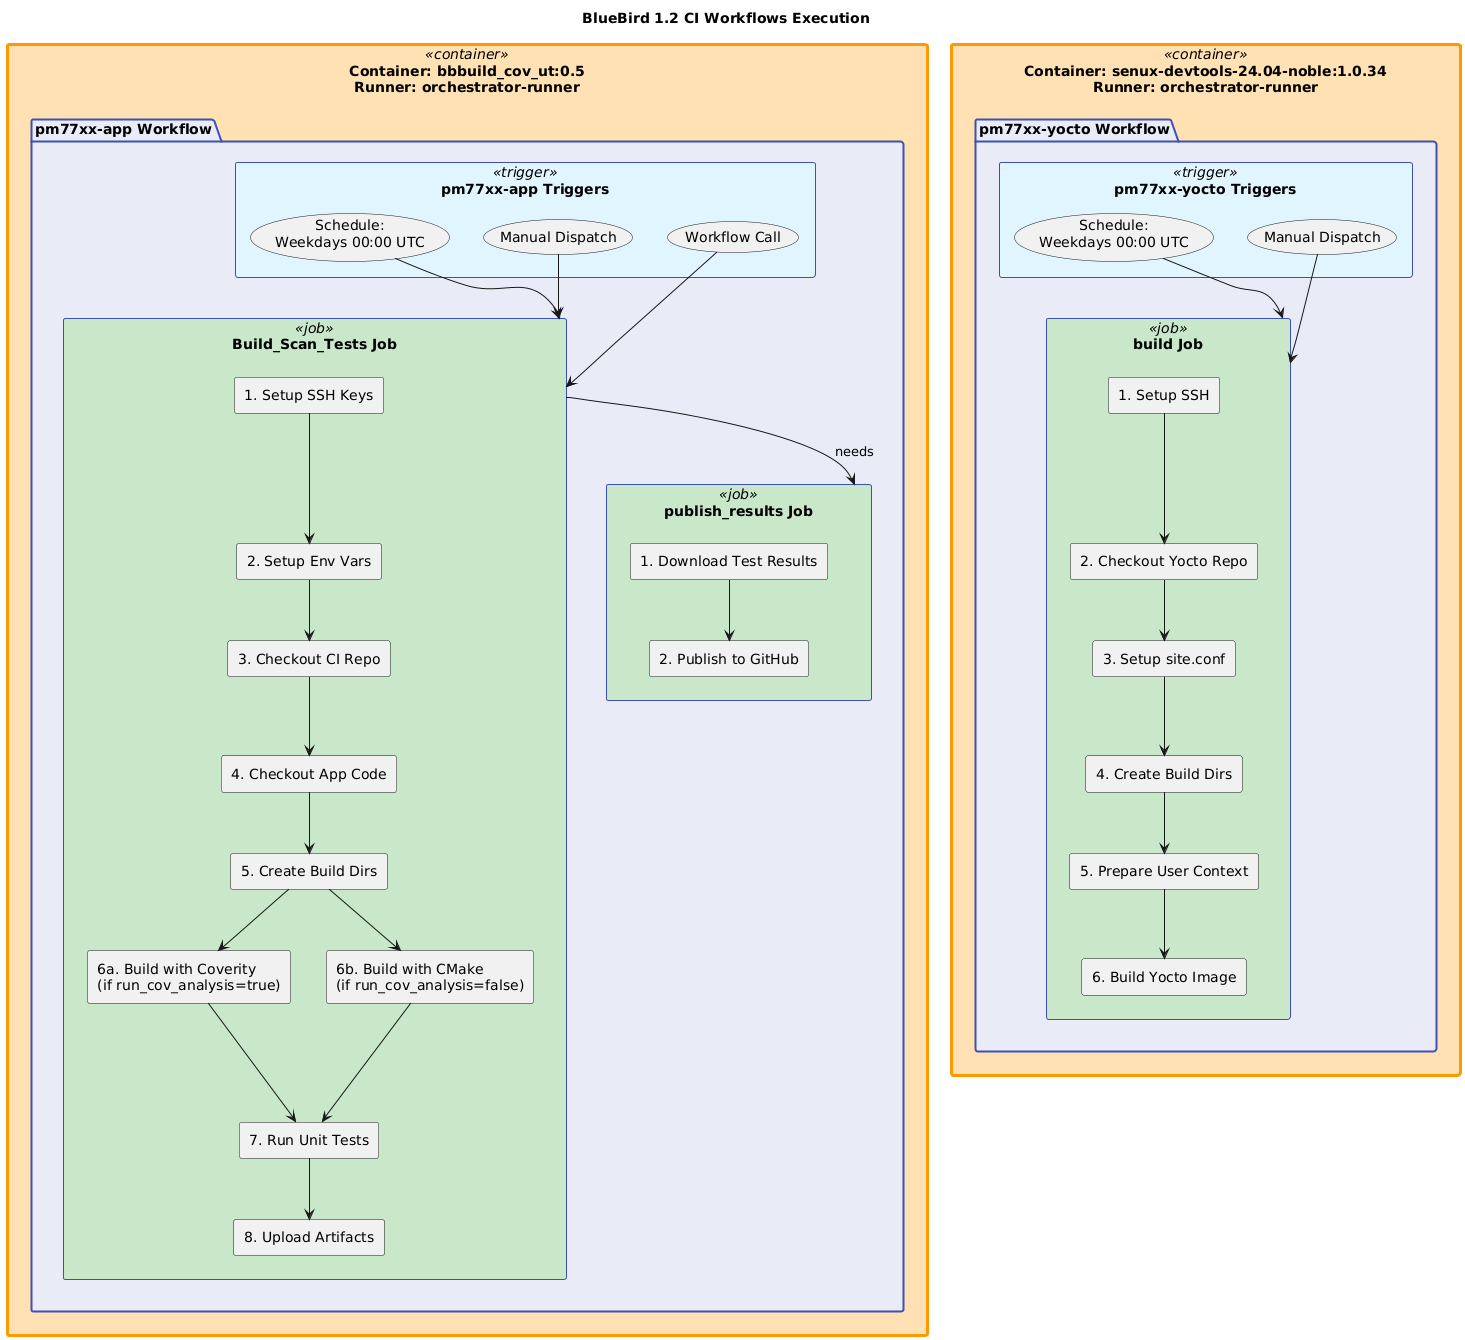
\includegraphics[width=\textwidth]{workflow-diagram}
\caption{Architecture générale de la chaîne d'intégration et de livraison}
\label{fig:bes-architecture}
\end{figure}

La figure~\ref{fig:bes-architecture} montre le flux. Un déclencheur (planifié
en jours ouvrés, manuel ou appel depuis un autre workflow) démarre un exécuteur
éphémère. Le job récupère l'image de compilation depuis Artifactory, puis, dans
ce conteneur, extrait trois dépôts : \texttt{bluebird/ci} (scripts),
\texttt{pm77xx-app/sdp} (code applicatif, sous-modules inclus) et
\texttt{pm77xx-app/automation-tests} (suites Robot Framework). Les cellules de
la matrice compilent, analysent et testent en parallèle ; les jobs aval
téléchargent l'archive produite, génèrent les rapports, soumettent l'archive de
production à BDBA, la publient dans Artifactory et envoient les métriques à
VictoriaMetrics, lues par Grafana.

Le tableau~\ref{tab:bes-herite-evolue} précise la part héritée et la part
apportée.

\begin{table}[H]
\centering
\caption{Situation à mon arrivée et évolutions apportées}
\label{tab:bes-herite-evolue}
\small
\begin{tabularx}{\textwidth}{@{}p{3.3cm} X X@{}}
\toprule
\textbf{Domaine} & \textbf{Existant} & \textbf{Évolution apportée} \\
\midrule
Compilation & Compilation de l'application &
  Matrice DEBUG/RELEASE $\times$ native amd64 / croisée aarch64 \\
Environnement & Image de compilation &
  Intégration du \gls{sdk} ; optimisation du \texttt{Dockerfile} ; mise à jour des paquets \\
Qualité & Analyse statique Coverity ; tests unitaires &
  Couverture (\texttt{gcovr}) et synthèse ; tests d'intégration Robot Framework \\
Sécurité & --- & Scan BDBA, rapport PDF et métriques \\
Livraison & Construction de la distribution &
  Publication des artefacts applicatifs, des images et du \gls{sdk} \\
Observabilité & Résultats par exécution &
  Action de collecte vers VictoriaMetrics ; mise à jour du tableau de bord Grafana \\
Infrastructure & Exécuteurs éphémères &
  Étude des solutions NFS et snapshot ; correction de scripts bash et Python \\
\bottomrule
\end{tabularx}
\end{table}

\subsection{Décomposition en chaînes}
\label{ssec:bes-chaines}

Le système comporte trois chaînes aux rythmes et aux durées différents
(tableau~\ref{tab:bes-chaines}). Le dépôt contient également un workflow
\texttt{evo-bench-image}, destiné aux images du banc de test ; il est hors du
périmètre de ce mémoire.

\begin{table}[H]
\centering
\caption{Chaînes d'intégration}
\label{tab:bes-chaines}
\small
\begin{tabularx}{\textwidth}{@{}l X p{4cm}@{}}
\toprule
\textbf{Chaîne} & \textbf{Objet} & \textbf{Déclenchement} \\
\midrule
\texttt{pm77xx-app} & Compilation, analyses, tests et publication de la couche applicative &
  Cron \texttt{0 0 * * 1-5}, manuel, appelé \\
\texttt{pm77xx-yocto} & Cinq variantes d'image et \gls{sdk} &
  Cron \texttt{0 22 * * 1-5}, manuel \\
\texttt{publish-image} & Construction, validation et publication de l'image de compilation &
  Manuel \\
\bottomrule
\end{tabularx}
\end{table}

La chaîne applicative est planifiée à minuit UTC et la chaîne Yocto à 22 h UTC :
elles ne se disputent donc pas les exécuteurs. Les durées mesurées sont
présentées au chapitre~\ref{chap:evaluation}.

La séparation s'impose pour trois raisons. Premièrement, les rythmes diffèrent :
le code applicatif change tous les jours alors que la distribution et l'image
de compilation évoluent rarement. Deuxièmement, les durées sont incompatibles :
intégrer une construction Yocto à plus d'une heure dans le chemin du développeur
dégraderait le retour d'information (ENF4). Troisièmement, les chaînes
s'articulent par des artefacts versionnés : le \gls{sdk} sort de
\texttt{pm77xx-yocto}, entre dans \texttt{publish-image}, et
\texttt{publish-image} appelle \texttt{pm77xx-app} comme sous-workflow pour
valider l'image candidate.

\begin{figure}[H]
\centering
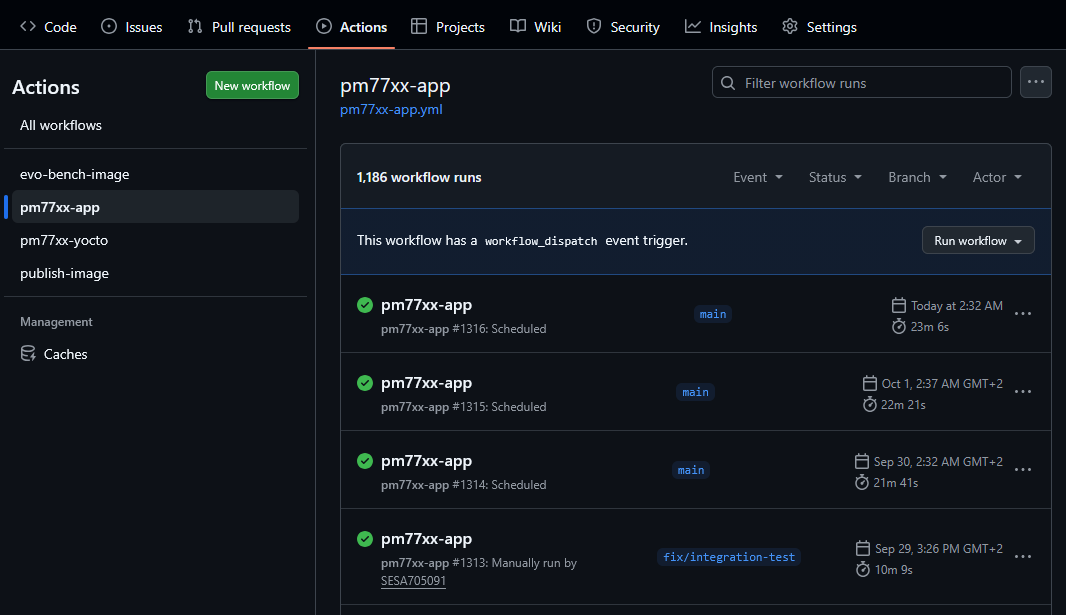
\includegraphics[width=\textwidth]{vue-global}
\caption{Historique des exécutions de \texttt{pm77xx-app} depuis la création du workflow (1\,186 exécutions)}
\label{fig:bes-historique}
\end{figure}

% ===========================================================================
\section{Mise en œuvre technique}
\label{sec:impl}

Chaque sous-section suit la même trame : l'objectif visé, l'état de départ,
l'évolution apportée, puis la difficulté rencontrée. Les références EF et ENF
renvoient aux exigences de la section précédente.

\subsection{Les chaînes CI}
\label{ssec:impl-chaines}

\subsubsection{Chaîne applicative \texttt{pm77xx-app}}
\label{sec:impl-pipeline-app}

\emph{Exigences : EF1 à EF9, ENF4, ENF5, ENF8, ENF9.}

\paragraph{Paramètres.} La chaîne accepte les entrées du
tableau~\ref{tab:impl-parametres-app} par \texttt{workflow\_dispatch} et
\texttt{workflow\_call}. Le mode appelé existe pour la validation de l'image de
compilation : \texttt{publish-image} appelle \texttt{pm77xx-app} en lui
passant l'étiquette candidate \texttt{bbbuild\_cov\_ut:test}, avec
\texttt{run\_cov\_analysis=false} pour éviter de polluer le serveur Coverity avec
une image non validée.

\begin{table}[H]
\centering
\caption{Paramètres d'entrée de \texttt{pm77xx-app}}
\label{tab:impl-parametres-app}
\small
\begin{tabularx}{\textwidth}{@{}l X l@{}}
\toprule
\textbf{Paramètre} & \textbf{Rôle} & \textbf{Défaut} \\
\midrule
\texttt{app\_repo\_branch} & Branche de \texttt{pm77xx-app/sdp} & \texttt{develop} \\
\texttt{test\_repo\_branch} & Branche de \texttt{automation-tests} & \texttt{main} \\
\texttt{builder\_img\_tag} & Image de compilation & \texttt{bbbuild\_cov\_ut:2.3} \\
\texttt{ci\_repo\_branch} & Branche de \texttt{bluebird/ci} & \texttt{main} \\
\texttt{run\_cov\_analysis} & Active la capture Coverity & \texttt{true} \\
\texttt{run\_robot\_tests} & Active les tests d'intégration & \texttt{false} \\
\texttt{workspace\_path} & Répertoire de travail dans le conteneur & \texttt{/\_\_w/ci/ci} \\
\bottomrule
\end{tabularx}
\end{table}

\paragraph{Matrice de construction.} La construction est déclinée selon
\texttt{build\_type} $\in$ \{DEBUG, RELEASE\} et \texttt{compiler\_type}
$\in$ \{amd64, aarch64\}, soit quatre cellules indépendantes
(\texttt{fail-fast: false}), exécutées en parallèle. Le
tableau~\ref{tab:impl-matrice-activites} répartit les activités sur ces
cellules ; cette répartition est un arbitrage entre coût et couverture.

\begin{table}[H]
\centering
\caption{Répartition des activités sur la matrice}
\label{tab:impl-matrice-activites}
\small
\begin{tabular}{@{}lcccc@{}}
\toprule
\textbf{Activité} & \makecell{DEBUG\\amd64} & \makecell{DEBUG\\aarch64} & \makecell{RELEASE\\amd64} & \makecell{RELEASE\\aarch64} \\
\midrule
Compilation            & \checkmark & \checkmark & \checkmark & \checkmark \\
Analyse statique       & --- & \checkmark & --- & --- \\
Tests unitaires        & \checkmark & --- & \checkmark & --- \\
Couverture             & \checkmark & --- & --- & --- \\
Tests d'intégration    & \checkmark$^{*}$ & --- & --- & --- \\
Analyse de composition & --- & --- & --- & \checkmark \\
Publication            & --- & --- & --- & \checkmark$^{\dagger}$ \\
\bottomrule
\end{tabular}

\smallskip
{\footnotesize $^{*}$ si \texttt{run\_robot\_tests=true}. $^{\dagger}$ sur la branche \texttt{main} uniquement.}
\end{table}

Les tests s'exécutent sur amd64 parce que le binaire s'exécute nativement sur
l'exécuteur ; les cellules aarch64 ne peuvent que compiler. La couverture
exige l'instrumentation \texttt{gcov}, donc un build DEBUG. L'analyse de
composition porte sur RELEASE/aarch64, c'est-à-dire sur l'artefact réellement
livré. Le listing~\ref{lst:impl-build} montre le point de bascule entre
compilation native et croisée.

\begin{lstlisting}[language=yaml,caption={Compilation native ou croisée selon la cellule de matrice},label={lst:impl-build}]
- name: Build ${{ matrix.compiler_type }} App in ${{ matrix.build_type }} mode
  id: build_app
  if: ${{ env.INPUT_RUN_COV_ANALYSIS == 'false'
       || matrix.build_type != 'DEBUG'
       || matrix.compiler_type != 'aarch64' }}
  run: |
    if [ "${{ matrix.compiler_type }}" == 'aarch64' ]; then
      . /usr/local/oecore-x86_64/environment-setup-aarch64-evo-linux
    fi
    cmake -DCMAKE_BUILD_TYPE=${{ matrix.build_type }} \
      -S "${{ env.SDP_ROOT }}" \
      -B "${{ env.SDP_ROOT }}/${{ matrix.build_type }}-build.${{ matrix.compiler_type }}"
    cmake --build "..." --parallel
\end{lstlisting}

La condition \texttt{if} rend cette étape exclusive de l'étape
\texttt{cov\_build\_app}, qui porte la condition inverse. Le répertoire de
build est suffixé par la configuration (\texttt{DEBUG-build.aarch64}), ce qui
évite toute collision entre cellules.

\begin{figure}[H]
\centering
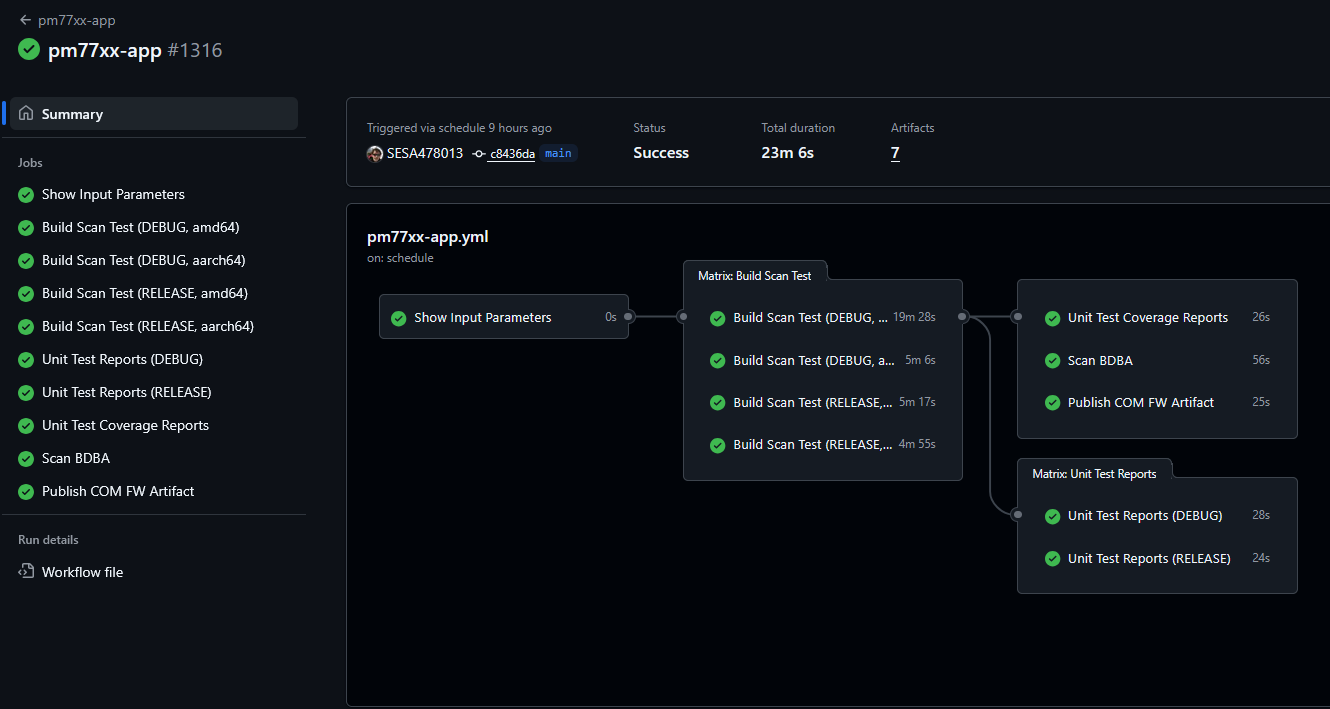
\includegraphics[width=0.95\textwidth]{workflow-pm77xx-app}
\caption{Exécution de \texttt{pm77xx-app} (\#1316) : matrice de construction et jobs aval}
\label{fig:impl-activite-app}
\end{figure}

La figure~\ref{fig:impl-activite-app} se lit de gauche à droite. Le job
\emph{Show Input Parameters} (0 s) écrit les paramètres dans la synthèse. Les
quatre cellules de la matrice démarrent ensuite : la cellule DEBUG/amd64 dure
19 min 28 s, contre 4 min 55 s à 5 min 17 s pour les trois autres ; elle
cumule la compilation instrumentée, les tests, la couverture et, si activés,
les tests d'intégration, et constitue donc le chemin critique des 23 min 06 s
de l'exécution. Les jobs aval (couverture 26 s, BDBA 56 s, publication 25 s,
rapports de test 28 s et 24 s) sont déclenchés dès la fin de la matrice
(\texttt{needs: build-scan-test}).

\paragraph{Difficulté : clonage multi-dépôts.} Le code est réparti entre un
dépôt principal et de nombreux sous-modules privés. Le checkout utilise
\texttt{submodules: recursive} avec la clé de service \texttt{GIT\_SRV\_SSH\_KEY}
et \texttt{persist-credentials: false}, de sorte que la clé ne reste pas dans
la configuration Git du répertoire de travail.

\subsubsection{Tests unitaires et couverture}
\label{ssec:impl-ut}

\emph{Exigences : EF5, EF7, EF8.}

\paragraph{Tests unitaires.} Les tests sont lancés par \texttt{ctest}, avec
export JUnit pour la publication, et excluent la suite \texttt{mcu\_unit\_tests},
destinée au cœur temps réel et inexécutable sur l'hôte :

\begin{lstlisting}[language=bash,caption={Exécution des tests unitaires},label={lst:impl-ctest}]
SDP_ROOT="$SDP_ROOT" ctest \
  --test-dir "$SDP_ROOT/${BUILD_TYPE}-build.${ARCH}" \
  --exclude-regex "mcu_unit_tests" \
  --output-on-failure \
  --output-junit "$SDP_ROOT/${BUILD_TYPE}-build.${ARCH}/test_results.xml"
\end{lstlisting}

L'étape est bornée par \texttt{timeout-minutes: 1} : un test qui ne rend jamais
la main ne doit pas immobiliser l'exécuteur jusqu'à la limite globale. Le job \texttt{test-reports} publie ensuite les
résultats avec l'action \texttt{EnricoMi/publish-unit-test-result-action}
(13 tests réussis sur 13 dans l'exécution \#1316).

\paragraph{Couverture.} La couverture est mesurée avec \texttt{gcovr} sur la
seule cellule DEBUG/amd64 :

\begin{lstlisting}[language=bash,caption={Mesure de couverture},label={lst:impl-gcovr}]
gcovr --root "$SDP_ROOT" --object-directory . \
  --exclude '.*/test/.*' \
  --gcov-ignore-parse-errors=negative_hits.warn \
  --html-details coverage/gcov.html \
  --lcov coverage/gcov.info \
  --json coverage/gcov.json \
  --json-summary coverage/gcov-summary.json \
  --print-summary | tee coverage/gcov-summary.txt
\end{lstlisting}

Trois choix sont à relever. L'option
\texttt{--gcov-ignore-parse-errors=negative\_hits.warn} dégrade en avertissement
les compteurs d'exécution négatifs produits par \texttt{gcov}, qui, sans cette
option, interrompent la génération du rapport. Les quatre formats de sortie répondent à quatre usages : HTML pour la
lecture, LCOV pour les outils tiers, JSON pour l'exploitation, texte pour la
synthèse. Enfin, le pourcentage de lignes est extrait par un filtre
\texttt{awk} sur la ligne \texttt{lines:} du résumé pour alimenter
VictoriaMetrics.

\texttt{gcov\_summary\_md.sh} convertit le résumé en tableau Markdown avec
badge et statut par métrique, selon deux seuils (50 \% et 75 \%). Sur le run
\#1316, la couverture est de 32,3 \% des lignes (19\,308 / 59\,772), 20,9 \% des
fonctions (1\,511 / 7\,216) et 29,6 \% des branches (5\,559 / 18\,775) ; les trois
indicateurs sont sous le seuil bas. La chaîne rend donc visible un niveau de
couverture faible plutôt que de le masquer.

\begin{figure}[H]
\centering
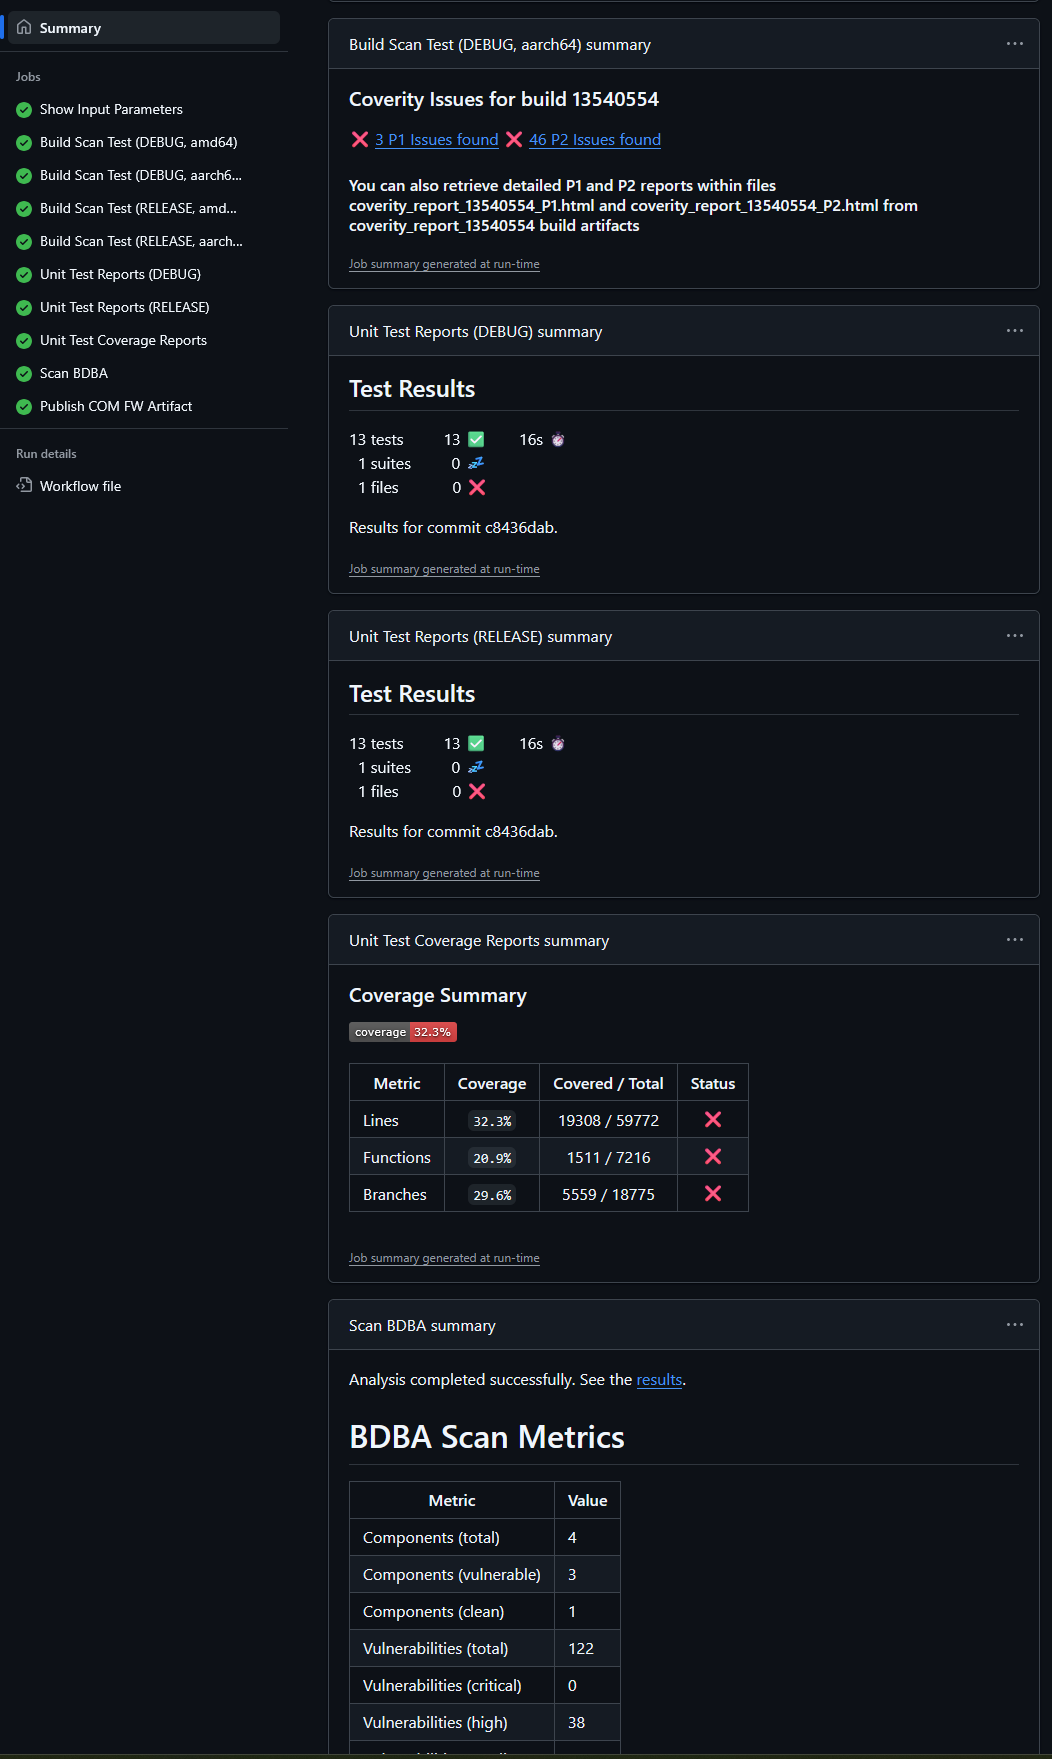
\includegraphics[width=0.75\textwidth]{summary-pm77xx-app}
\caption{Synthèse d'exécution : défauts Coverity, tests, couverture et BDBA}
\label{fig:impl-synthese}
\end{figure}

\paragraph{Difficulté : chemins d'artefacts.} \texttt{upload-artifact} conserve
l'arborescence absolue du conteneur. Le job \texttt{ut-coverage-reports}, qui
s'exécute dans une autre image, doit donc retrouver les fichiers sous
\texttt{./build-amd64/\_\_w/ci/ci/pm77xx/pm77xx-app/sdp/DEBUG-build.amd64}.
Ce chemin est centralisé dans une variable \texttt{BUILD\_PATH} pour limiter sa
duplication.

\subsubsection{Tests d'intégration Robot Framework}
\label{ssec:impl-robot}

\emph{Exigence : EF6.}

Les suites Robot Framework du dépôt \texttt{automation-tests} exercent les
services applicatifs. Leur exécution est un ajout récent. Elle est désactivée par
défaut (\texttt{run\_robot\_tests=false}) et ne concerne que la cellule
DEBUG/amd64, car le lanceur de services attend les binaires de l'arborescence
x86\_64/DEBUG. La séquence, entièrement conditionnée à \texttt{steps.launch\_sdp.outcome}, est la suivante :

\begin{enumerate}[nosep]
  \item \texttt{cmake --install} copie configuration, scripts de migration de base
        de données et certificats sous \texttt{/opt/app-ext/sdp} ;
  \item \texttt{sdp.launch.in.container.sh} démarre les services en arrière-plan
        (\texttt{timeout-minutes: 5}) ;
  \item \texttt{robot} produit \texttt{output.xml}, \texttt{log.html},
        \texttt{report.html} et \texttt{xunit.xml} ;
  \item \texttt{sdp.launch.in.container.sh --kill} arrête les services dans une
        étape \texttt{if: always()}, même si les tests ont échoué ;
  \item \texttt{robot\_summary\_md.py} écrit la synthèse (badge de taux de
        réussite, compteurs, 50 échecs listés au plus) dans le résumé du run.
\end{enumerate}

La difficulté principale est d'exécuter un ensemble de services système
(\texttt{dbus}, services dépendant de \texttt{libsystemd}) dans un conteneur sans
gestionnaire de services complet. Le lanceur démarre donc chaque service
lui-même et la garde de 5 minutes protège contre un service qui resterait au
premier plan.

\subsubsection{Analyse statique Coverity}
\label{ssec:impl-coverity}

\emph{Exigence : EF3.}

Coverity préexistait ; mon travail a porté sur la fiabilisation des scripts et
sur la restitution. L'analyse suit trois phases pilotées par
\texttt{cov\_build.sh \{capture|analyze|commit\}}, chacune dans une étape
distincte afin d'isoler les échecs et de mesurer chaque durée. La configuration
\texttt{scripts/coverity\_ci.yaml} active tous les vérificateurs, y compris la
famille de sécurité C :

\begin{lstlisting}[language=yaml,caption={Configuration Coverity},label={lst:impl-cov-config}]
capture:
  build:
    cov-build-args: [--parallel-translate=4]
analyze:
  c-cpp-virtual: true
  c-cpp-fnptr: true
  checkers: { all: true, rule: true, c-family-security: true }
  cov-analyze-args:
    - --strip-path
    - /__w/ci/ci/pm77xx/pm77xx-app/
commit:
  connect:
    stream: "<flux-projet>"
    url: "https://<serveur-coverity>"
\end{lstlisting}

\texttt{c-cpp-virtual} et \texttt{c-cpp-fnptr} résolvent les appels virtuels
et les pointeurs de fonction, nombreux dans le code applicatif.
\texttt{--strip-path} supprime le préfixe du répertoire de travail afin que
l'identité d'un défaut (fichier, fonction, type) reste stable d'un run à l'autre
malgré des exécuteurs éphémères (ENF20). Sans lui, un même défaut serait
compté comme nouveau à chaque modification du chemin.

\paragraph{Restitution ciblée.} \texttt{extract\_cov.sh} interroge, pour chacune
des vues P1 et P2, l'API REST
\texttt{/api/v2/streams/viewContents/\{viewid\}} via \texttt{pyCovXtract.py},
génère les rapports \texttt{coverity\_report\_<run>\_P1.html} et
\texttt{\_P2.html}, et expose \texttt{cov\_p1\_issue\_nbr},
\texttt{cov\_p2\_issue\_nbr} et \texttt{cov\_total\_issue\_nbr} dans
\texttt{GITHUB\_OUTPUT}. Sur le run \#1316 : 3 défauts P1 et 46 défauts P2.

\paragraph{Politique de blocage.} Le script retourne 1 lorsque des défauts sont
trouvés. L'étape l'invoque avec \texttt{|| true}, car un code de sortie non nul
colorait l'étape en rouge alors que le résultat est déjà exposé dans la
synthèse. Seuls un échec de capture, d'analyse ou de connexion fait donc échouer
le job. Ce choix est assumé : avec une dette initiale de 46 défauts P2, un
blocage immédiat paralyserait l'équipe. La trajectoire cible est un blocage sur
les défauts nouvellement introduits uniquement, ce que l'option \texttt{--diff}
de \texttt{pyCovXtract.py} permettrait de calculer.

\subsubsection{Analyse de composition BDBA}
\label{ssec:impl-bdba}

\emph{Exigence : EF4.}

Le job \texttt{scan-bdba} télécharge l'archive RELEASE/aarch64 puis enchaîne
trois étapes :

\begin{enumerate}[nosep]
  \item soumission par \texttt{Foxy/action-bdba-scan@v1.1.1}
        (\texttt{delete-binary: true}, produit \texttt{pm77xx-app} version 1.0.0) ;
  \item \texttt{BDBA\_GetReport.py} interroge \texttt{/api/product/\{id\}/} toutes
        les 30 s jusqu'au statut \texttt{R} (délai maximal de 600 s) puis télécharge
        le rapport PDF ;
  \item \texttt{BDBA\_ExtractMetrics.py} produit un fichier JSON Lines au format
        d'import VictoriaMetrics, et expose les compteurs
        \texttt{bdba\_components\_total}, \texttt{bdba\_components\_vuln},
        \texttt{bdba\_vulns\_total}, \texttt{bdba\_vulns\_critical},
        \texttt{bdba\_vulns\_high}, \texttt{bdba\_vulns\_medium},
        \texttt{bdba\_vulns\_low}.
\end{enumerate}

Le tableau~\ref{tab:impl-bdba-metriques} définit les indicateurs. Sur
l'exécution capturée (figure~\ref{fig:impl-bdba}), BDBA identifie 4 composants
dont 3 vulnérables (\texttt{cjson}, \texttt{openldap}, \texttt{hostapd}) pour
122 vulnérabilités : 5 critiques, 19 élevées, 86 moyennes et 12 faibles. Les
compteurs BDBA de la synthèse (figure~\ref{fig:impl-synthese}) proviennent d'une
autre exécution et diffèrent donc légèrement ; ce mémoire retient les valeurs
du rapport.

\begin{table}[H]
\centering
\caption{Indicateurs extraits de l'analyse de composition}
\label{tab:impl-bdba-metriques}
\small
\begin{tabularx}{\textwidth}{@{}l X@{}}
\toprule
\textbf{Indicateur} & \textbf{Définition} \\
\midrule
\texttt{bdba\_component} & Composants tiers détectés, étiquetés \texttt{vulnerable} ou \texttt{clean} \\
\texttt{bdba\_vulns} & Vulnérabilités connues, étiquetées par sévérité \\
\bottomrule
\end{tabularx}
\end{table}

\begin{figure}[H]
\centering
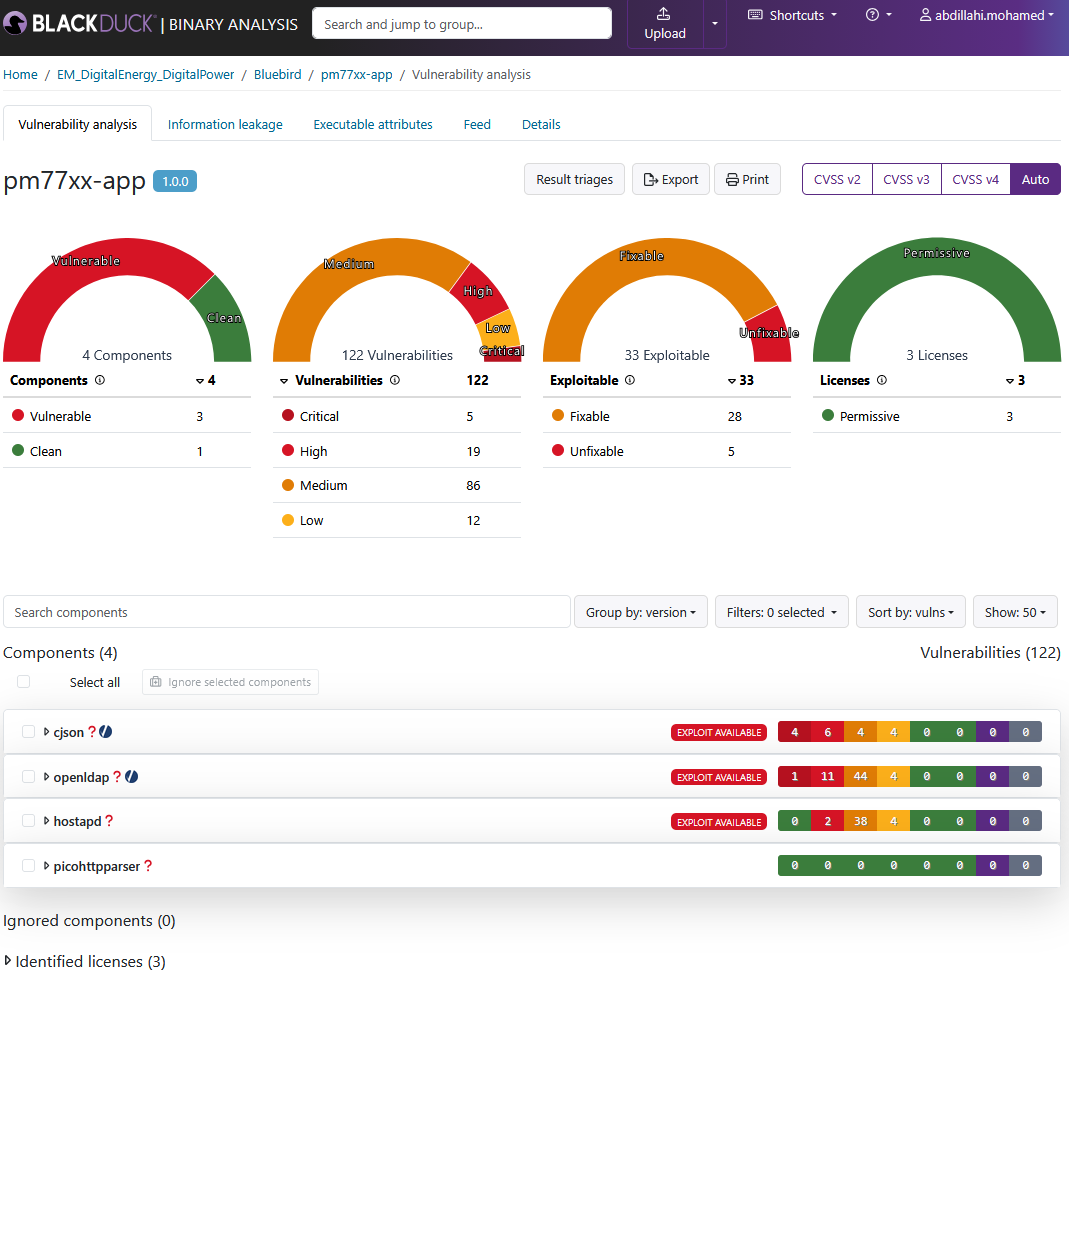
\includegraphics[width=0.7\textwidth]{rapport-bdba}
\caption{Rapport BDBA de l'archive \texttt{pm77xx-app} (RELEASE/aarch64)}
\label{fig:impl-bdba}
\end{figure}

Cette analyse alimente l'inventaire des composants que les obligations de
nomenclature logicielle exigent (section~\ref{sec:art-supply-chain}).

\subsubsection{Publication des artefacts applicatifs}
\label{ssec:impl-publication-app}

\emph{Exigence : EF9.}

Chaque cellule empaquette son résultat avant de le publier :
\texttt{DESTDIR=/tmp/staging cmake --install} installe dans une arborescence
temporaire, puis \texttt{tar -czf} archive \texttt{lib} et \texttt{bin} depuis
\texttt{/opt/app-ext/sdp}. L'archive est conservée comme artefact de run
(\texttt{<BUILD>-build-<ARCH>}). Pour la branche \texttt{main}, le job
\texttt{upload-artifact} publie l'archive RELEASE/aarch64 dans Artifactory par
\texttt{jf rt upload} dans le répertoire \texttt{sdp-artifacts/} du dépôt
générique, sous un nom de la forme
\texttt{pm77xx-app-artifact-<version>-<horodatage>.tar.gz}.
La taille de l'archive est aussi mesurée (\texttt{du -cb}) et envoyée comme
métrique \texttt{sdp\_artifact\_size} (78,0 Mo sur la capture du tableau de bord).

\emph{Limite :} la version \texttt{ARTIFACT\_VERSION} est fixée à \texttt{0.0.1} ;
seul l'horodatage distingue deux artefacts, et le nom ne contient ni
l'empreinte du commit ni la version de l'image de compilation. L'exigence EF9
n'est donc que partiellement couverte.

\subsubsection{Chaîne de la distribution \texttt{pm77xx-yocto}}
\label{sec:impl-pipeline-yocto}

\emph{Exigences : EF10 à EF13, ENF6.}

La configuration est décrite avec kas 5.2 en trois niveaux, composés dans la
ligne de commande par des « : » :

\begin{lstlisting}[language=bash,caption={Appels kas : image et SDK},label={lst:impl-kas}]
kas build kas/board/<carte>.yml:kas/project/image-evo-dev.yml
kas build kas/board/<carte>.yml:kas/project/image-evo-dev.yml:\
         kas/project/option/populate-sdk.yml
\end{lstlisting}

Le premier niveau décrit la carte (\Carte), le second
le projet d'image, le troisième des options, dont \texttt{populate-sdk.yml}.
Pour la variante de production, le fichier de carte est suffixé
(\texttt{<carte>-prod.yml}) grâce à l'entrée \texttt{include} de la matrice.
Les cinq variantes (tableau~\ref{tab:impl-variantes}) sont construites en
parallèle.

\begin{table}[H]
\centering
\caption{Variantes d'image produites}
\label{tab:impl-variantes}
\small
\begin{tabularx}{\textwidth}{@{}l X@{}}
\toprule
\textbf{Variante} & \textbf{Usage} \\
\midrule
\texttt{image-evo-dev} & Développement, outils de débogage ; sert aussi à générer le \gls{sdk} \\
\texttt{image-evo-hwtest} & Validation matérielle en production \\
\texttt{image-evo-netboot} & Démarrage réseau (initramfs) \\
\texttt{image-evo-rescue} & Image de secours (initramfs) \\
\texttt{image-evo-prod} & Production \\
\bottomrule
\end{tabularx}
\end{table}

\begin{figure}[H]
\centering
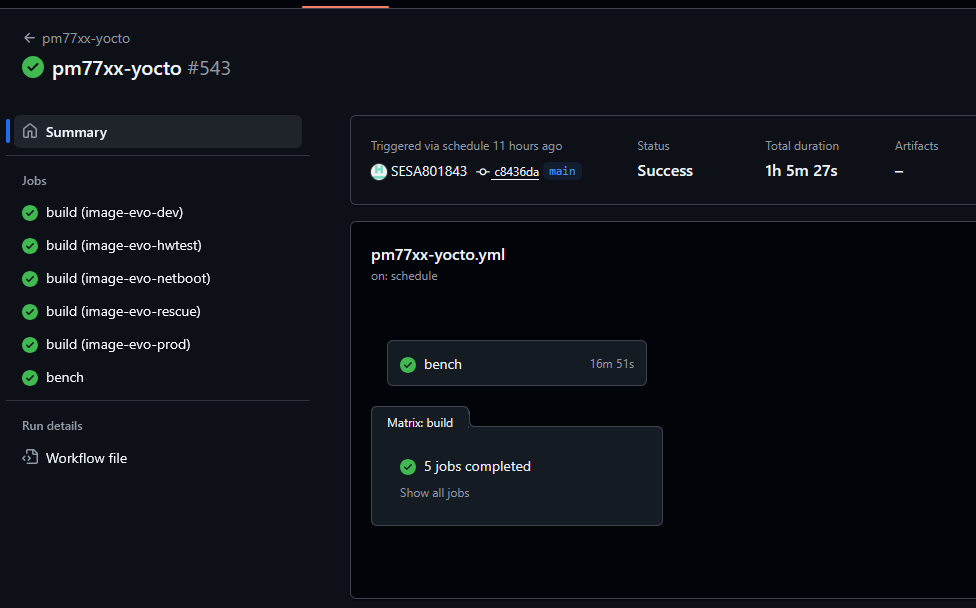
\includegraphics[width=0.6\textwidth]{workflow-pm77xx-yocto}
\caption{Exécution de \texttt{pm77xx-yocto} (\#543, 1 h 05 min 27 s)}
\label{fig:impl-yocto}
\end{figure}

\paragraph{Difficulté : BitBake refuse de s'exécuter en root.} Le conteneur
est imposé en root par l'infrastructure (section~\ref{ssec:impl-runners}), or
BitBake refuse de s'exécuter sous cet utilisateur. Le workflow écrit donc la clé
SSH sous \texttt{/home/user/.ssh}, transfère la propriété du répertoire de
travail à \texttt{user} (\texttt{chown -R}), déclare le dépôt en
\texttt{safe.directory} puis lance \texttt{kas} par \texttt{su user -c}.

\paragraph{Publication.} Après la construction, le \gls{sdk} est localisé par
\texttt{find build/*tmp*/deploy/sdk -name '*-toolchain-*.sh'} puis publié dans
\texttt{sdk/} ; les variantes \texttt{dev} et \texttt{prod} sont archivées
(\texttt{find -type f | tar --transform 's|.*/||'} met tous les fichiers à la racine de
l'archive) et publiées dans \texttt{bsp-images/}. Pour la variante dev, une
archive « flashable » regroupe \texttt{deploy/images} et le fichier machine
\texttt{<carte>.conf} dans \texttt{bsp-images/standalone-flashing-images/}.
Un développeur applicatif obtient ainsi un compilateur croisé et une image de
référence sans reconstruire la distribution.

\begin{figure}[H]
\centering
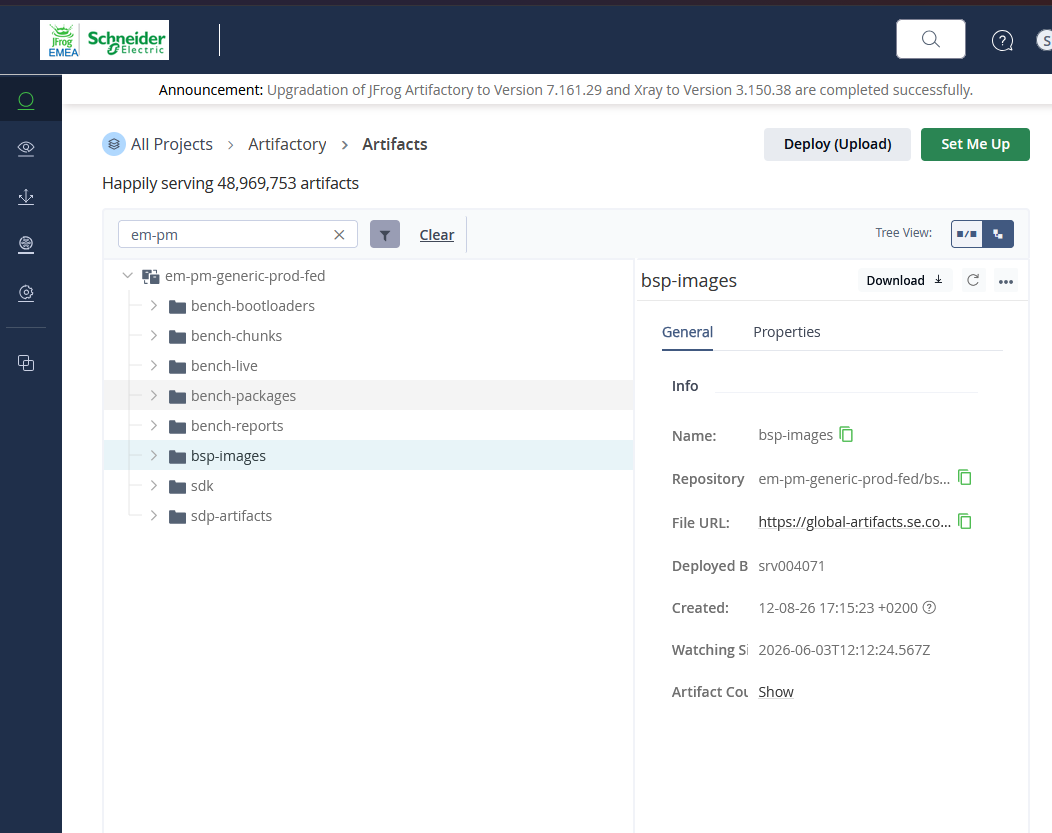
\includegraphics[width=0.75\textwidth]{jfrog-artifactory}
\caption{Organisation du dépôt générique Artifactory}
\label{fig:impl-artifactory}
\end{figure}

\subsubsection{Chaîne de l'image de compilation \texttt{publish-image}}
\label{sec:impl-conteneur}

\emph{Exigences : EF14 à EF17, ENF1, ENF2, ENF12.}

\paragraph{Construction du \texttt{Dockerfile}.} L'image est construite en trois
étages à partir d'une image Ubuntu 24.04 (\texttt{se-ubuntu-noble:3.0.1}) :
\texttt{compiler} (paquets et compilateurs), \texttt{cov-sdk\_builder}
(Coverity et \gls{sdk}) et \texttt{app\_builder} (image finale). Seul le contenu
utile est copié dans l'étage final (\texttt{COPY --from=cov-sdk\_builder}), de sorte que l'archive
Coverity et l'installateur du \gls{sdk} n'alourdissent pas l'image.

\begin{table}[H]
\centering
\caption{Principaux composants de l'image et versions épinglées}
\label{tab:impl-image-versions}
\small
\begin{tabularx}{\textwidth}{@{}l X l@{}}
\toprule
\textbf{Composant} & \textbf{Rôle} & \textbf{Version} \\
\midrule
GCC / G++ & Compilation C et C++ & 13.3.0-6ubuntu2\textasciitilde 24.04.1 \\
CMake & Système de construction & 3.28.3-1build7 \\
Meson / Ninja & Brique de cybersécurité (csb-app) & 1.3.2 / 1.11.1 \\
Coverity Analysis & Analyse statique & 2024.12.0 \\
GoogleTest / GMock & Tests unitaires & 1.14.0-1 \\
CMocka & Doublures de dépendances & 1.1.7-3 \\
gcovr & Couverture & 7.0-1 \\
Doxygen / Graphviz & Documentation & 1.9.8 / 2.42.2 \\
Python & Scripts d'intégration continue & 3.12.3 \\
\bottomrule
\end{tabularx}
\end{table}

Les optimisations apportées sont les suivantes :

\begin{itemize}[nosep]
  \item versions épinglées par paquet (\texttt{cmake=3.28.3-1build7}), pour que deux
        constructions séparées dans le temps utilisent la même chaîne d'outils (ENF1) ;
  \item \texttt{--no-install-recommends}, qui évite l'installation de paquets non demandés ;
  \item caches BuildKit \texttt{--mount=type=cache,target=/var/cache/apt} et
        \texttt{/var/lib/apt} (\texttt{sharing=locked}) : les paquets déjà téléchargés
        sont réutilisés d'une construction à l'autre sans rester dans une couche ;
  \item construction multi-étages, décrite plus haut.
\end{itemize}

\paragraph{Accès aux dépôts privés.} La brique de cybersécurité \texttt{csb-app}
(version \texttt{Release\_csbApp\_2.6.0}) est clonée et compilée avec Meson dans
l'image. Le clonage utilise \texttt{RUN --mount=type=ssh}, alimenté par
\texttt{docker build --ssh default} : la clé reste dans l'agent SSH de l'hôte et
n'est écrite dans aucune couche de l'image.

\begin{lstlisting}[language=docker,caption={Installation du SDK et clonage sécurisé},label={lst:impl-dockerfile}]
COPY ./resources/*sdk-installer*.sh ${SDK_PATH}/sdk-installer.sh
RUN chmod +x sdk-installer.sh \
    && ./sdk-installer.sh -d /usr/local/oecore-x86_64 -y

RUN --mount=type=ssh \
    ssh-keyscan <forge-interne> >> /root/.ssh/known_hosts \
    && git clone --branch Release_csbApp_2.6.0 \
       git@<forge-interne>:<organisation>/csb-app.git csb-app
\end{lstlisting}

L'image définit l'utilisateur \texttt{user}, mais son exécution en
intégration se fait en root (\texttt{options: -u root}) pour des raisons de
droits d'écriture imposées par RaaS ; ce point est reporté en perspectives.

\begin{figure}[H]
\centering
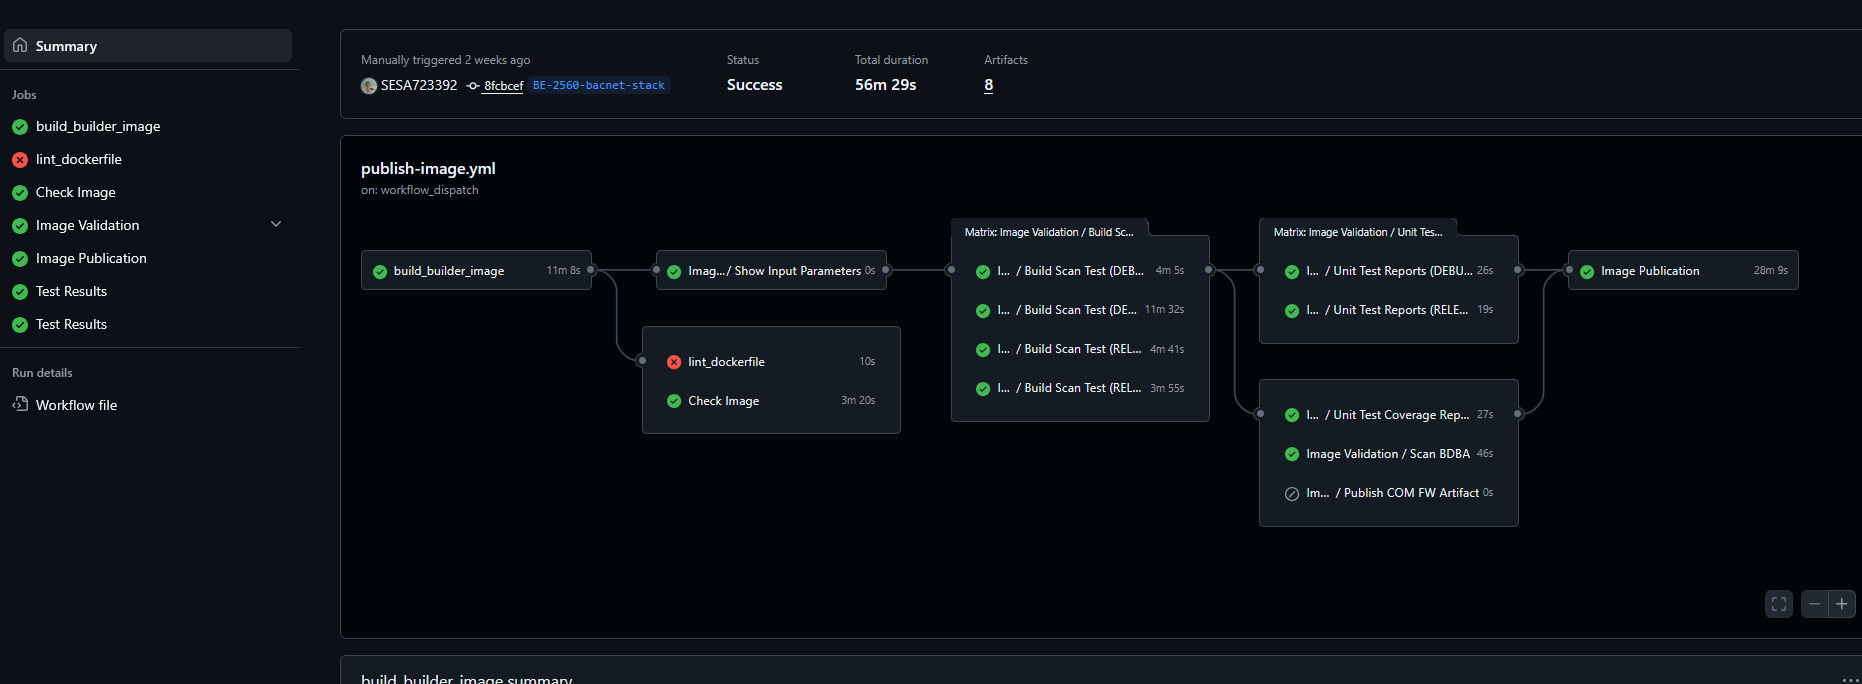
\includegraphics[width=\textwidth]{workflow-image-docker}
\caption{Exécution de \texttt{publish-image} : construction, contrôles, validation, publication}
\label{fig:impl-cycle-image}
\end{figure}

\paragraph{Cycle de validation.} La figure~\ref{fig:impl-cycle-image} détaille
l'enchaînement :
\begin{enumerate}[nosep]
  \item \texttt{build\_builder\_image} (11 min 08 s) construit avec
        \texttt{DOCKER\_BUILDKIT=1 docker build --ssh default --build-arg COV\_VERSION=2024.12.0}
        et pousse l'image \texttt{:test} ;
  \item \texttt{lint\_dockerfile} exécute \texttt{hadolint}, et \texttt{Check Image}
        (3 min 20 s) lance \texttt{display\_version.sh} dans l'image pour vérifier la
        présence et les versions des outils (EF15) ;
  \item \emph{Image Validation} appelle \texttt{pm77xx-app} avec
        \texttt{builder\_img\_tag=bbbuild\_cov\_ut:test} : quatre cellules de
        compilation, rapports de test, couverture et BDBA ;
  \item \emph{Image Publication} (28 min 09 s) revérifie l'étiquette, republie
        l'image sous son étiquette définitive et en exporte une archive.
\end{enumerate}

Une image n'atteint donc l'étiquette définitive qu'après avoir prouvé qu'elle
construit le produit. Sur la capture, le job \texttt{lint\_dockerfile} est en
échec alors que l'exécution se termine en succès : les erreurs de \texttt{hadolint}
sont tolérées. C'est un choix provisoire, le temps de résorber les
avertissements existants.

% ===========================================================================
\subsection{L'infrastructure d'exécution}
\label{ssec:impl-runners}

\emph{Exigences : ENF4, ENF6, ENF19 à ENF21.}

\subsubsection{Modèle d'exécuteurs éphémères}

Les jobs lourds (compilation, Yocto, construction d'image) s'exécutent sur
\texttt{orchestrator-runner}, un service d'exécuteurs qui alloue une machine
neuve par job et la détruit ensuite. Les jobs légers (rapports de test, couverture, BDBA,
publication) utilisent \texttt{ubuntu-22.04} avec l'image
\texttt{se-ubuntu-noble:3.0.1} : ils n'ont pas besoin de la chaîne d'outils et
ne doivent pas occuper un exécuteur coûteux. Les contraintes générales de ce
modèle sont décrites en section~\ref{sssec:bes-contraintes-infra} ; leur
traduction dans la chaîne est la suivante :

\begin{itemize}[nosep]
  \item \textbf{Droits.} Le conteneur est lancé avec \texttt{options: -u root},
        ce qui oblige la chaîne Yocto à rétrograder les privilèges
        (section~\ref{sec:impl-pipeline-yocto}).
  \item \textbf{Chemins.} Le répertoire de travail \texttt{/\_\_w/ci/ci} est
        paramétré (\texttt{workspace\_path}) et neutralisé côté Coverity par
        \texttt{--strip-path}.
  \item \textbf{Temps.} Des garde-fous \texttt{timeout-minutes} limitent les étapes
        susceptibles de bloquer.
\end{itemize}

\subsubsection{Limite : le cache de la distribution}

Les répertoires \texttt{DL\_DIR} et \texttt{SSTATE\_DIR} sont créés dans
l'espace de travail du job par un fichier \texttt{site.conf} généré à
l'exécution :

\begin{lstlisting}[language=bash,caption={Configuration Yocto générée par le job},label={lst:impl-siteconf}]
DL_DIR     = '$GITHUB_WORKSPACE/projets/yocto/downloads'
SSTATE_DIR = '$GITHUB_WORKSPACE/projets/yocto/sstate-cache'
BB_NUMBER_THREADS = '32'
PARALLEL_MAKE = '-j 32'
\end{lstlisting}

L'exécuteur étant détruit à la fin du job, ces deux caches repartent de zéro à
chaque exécution : chacune des cinq variantes retélécharge les sources et
recompile l'ensemble des paquets, ce qui explique en grande partie la durée de
1 h 05 de la chaîne. La parallélisation à 32 threads ne réduit que la durée de
chaque compilation, pas la redondance entre cellules. L'exigence ENF6
(cache partagé) n'est donc \emph{pas} couverte par la chaîne actuelle.

\subsubsection{Étude des solutions NFS et snapshot}
\label{sssec:impl-etude-cache}

J'ai étudié deux solutions pour rendre ces caches persistants malgré le caractère
éphémère des exécuteurs (tableau~\ref{tab:impl-cache}).

\begin{table}[H]
\centering
\caption{Solutions étudiées pour le cache de la distribution}
\label{tab:impl-cache}
\small
\begin{tabularx}{\textwidth}{@{}p{2.6cm} X X@{}}
\toprule
\textbf{Solution} & \textbf{Principe} & \textbf{Points d'attention} \\
\midrule
Partage NFS &
  Montage d'un volume réseau comme \texttt{DL\_DIR} et \texttt{SSTATE\_DIR} &
  Écritures concurrentes des cinq cellules de la matrice ; latence sur de très
  nombreux petits fichiers ; disponibilité du service depuis les exécuteurs \\
Snapshot &
  Volume restauré au démarrage de l'exécuteur à partir d'un instantané du cache &
  Instantané à rafraîchir régulièrement ; cache en lecture seule, les nouveaux
  états n'étant pas réinjectés ; compatibilité avec le service d'exécuteurs \\
\bottomrule
\end{tabularx}
\end{table}

\paragraph{Conclusion de l'étude.} La solution retenue est le partage NFS. Le
snapshot ne fournit qu'un cache en lecture seule, figé à la date de
l'instantané : les états produits par une exécution ne profitent pas aux
suivantes tant que l'instantané n'est pas régénéré. Un volume NFS, au contraire,
est alimenté à chaque construction et reste à jour sans opération
supplémentaire. Le principal point à traiter lors de la mise en œuvre est la
gestion des écritures concurrentes des cinq cellules de la matrice. Cette
solution n'est pas encore mise en œuvre ; elle constitue la première perspective
de ce travail (section~\ref{sec:concl-perspectives}).

\subsubsection{Gestion des secrets et sécurité}

Les secrets utilisés sont \texttt{GIT\_SRV\_SSH\_KEY}, \texttt{COV\_AUTH\_JSON},
\texttt{COV\_SRV\_CNXON}, \texttt{AM\_BDBA\_API\_TOKEN}, \texttt{JFROG\_SRV\_PAT} et
\texttt{VMET\_PASSWORD}. Les fichiers qui les contiennent sont créés avec
\texttt{chmod 0600} et supprimés après usage (\texttt{.cov\_cnx.yml}), le
checkout n'enregistre pas les identifiants (\texttt{persist-credentials: false})
et l'image de compilation ne contient aucune clé grâce au montage SSH. Deux
limites subsistent : le jeton BDBA est passé en argument de ligne de commande
aux scripts Python, donc visible dans la liste des processus de l'exécuteur
(masqué dans les journaux, mais pas dans la machine) ; et la chaîne Yocto écrit
la clé SSH sur le disque de l'exécuteur, dans un répertoire détruit avec lui.

% ===========================================================================
\subsection{L'observabilité}
\label{ssec:impl-observabilite}

\emph{Exigences : EF18 à EF22, ENF15 à ENF18.}

La synthèse d'un run ne montre pas de tendance. Pour suivre la qualité dans le
temps, chaque chaîne envoie ses indicateurs à VictoriaMetrics, qu'un tableau de
bord Grafana interroge.

\paragraph{Action de collecte.} L'action composite
\texttt{.github/actions/upload-vm-metrics} encapsule l'envoi pour éviter de
dupliquer les appels \texttt{curl} dans chaque workflow. Elle accepte deux
modes, selon la source :

\begin{lstlisting}[language=bash,caption={Deux modes d'envoi des métriques},label={lst:impl-vm}]
# Mode fichier : JSON Lines d'import (BDBA, plusieurs séries)
curl -T "$METRICS_JSONL_FILE" -u "$VMET_USER:$VMET_PASSWORD" \
     -X POST "https://$VMET_URL/api/v1/import"

# Mode valeur unique : format texte Prometheus
curl -d "${METRIC_NAME}{${METRIC_LABELS}} ${METRIC_VALUE}" \
     -u "$VMET_USER:$VMET_PASSWORD" \
     -X POST "https://$VMET_URL/api/v1/import/prometheus"
\end{lstlisting}

Le mode texte suffit pour une valeur scalaire (taille de l'artefact,
couverture) ; le mode JSON Lines est nécessaire quand un script produit
plusieurs séries étiquetées (\texttt{bdba\_component} par statut,
\texttt{bdba\_vulns} par sévérité). Les étiquettes communes
(\texttt{bu="em"}, \texttt{project="bluebird"}, \texttt{repo},
\texttt{branch}, \texttt{workflow}) permettent de filtrer par chaîne et par
branche dans Grafana. Le nom d'utilisateur est une variable de dépôt et le mot de
passe un secret.

\begin{table}[H]
\centering
\caption{Indicateurs collectés vers VictoriaMetrics}
\label{tab:impl-indicateurs}
\small
\begin{tabularx}{\textwidth}{@{}l X l@{}}
\toprule
\textbf{Métrique} & \textbf{Contenu} & \textbf{Origine} \\
\midrule
\texttt{sdp\_artifact\_size} & Taille de l'archive \texttt{lib} + \texttt{bin} & \texttt{du -cb}, chaque cellule \\
\texttt{code\_coverage} & Couverture de lignes (\%) & \texttt{gcovr}, DEBUG/amd64 \\
\texttt{bdba\_component} & Composants, par statut & \texttt{BDBA\_ExtractMetrics.py} \\
\texttt{bdba\_vulns} & Vulnérabilités, par sévérité & \texttt{BDBA\_ExtractMetrics.py} \\
\bottomrule
\end{tabularx}
\end{table}

\paragraph{Tableau de bord.} J'ai mis à jour le tableau de bord Grafana
« Bluebird w1.2 / Daily -- COM team » (figure~\ref{fig:impl-grafana}). Il est
organisé en quatre sections : sprint en cours, \emph{Quality \& Security}
(défauts Coverity P1 et P2, couverture, taille de l'artefact, répartition des
composants et des vulnérabilités), état des workflows (statut et durée du
dernier run, un onglet par chaîne) et pull requests ouvertes. À la date de la
capture, il affiche 3 défauts P1, 46 défauts P2, 32,3 \% de couverture, un
artefact de 78,0 Mo et un dernier run \texttt{pm77xx-app} réussi en 23,1 minutes.

\begin{figure}[H]
\centering
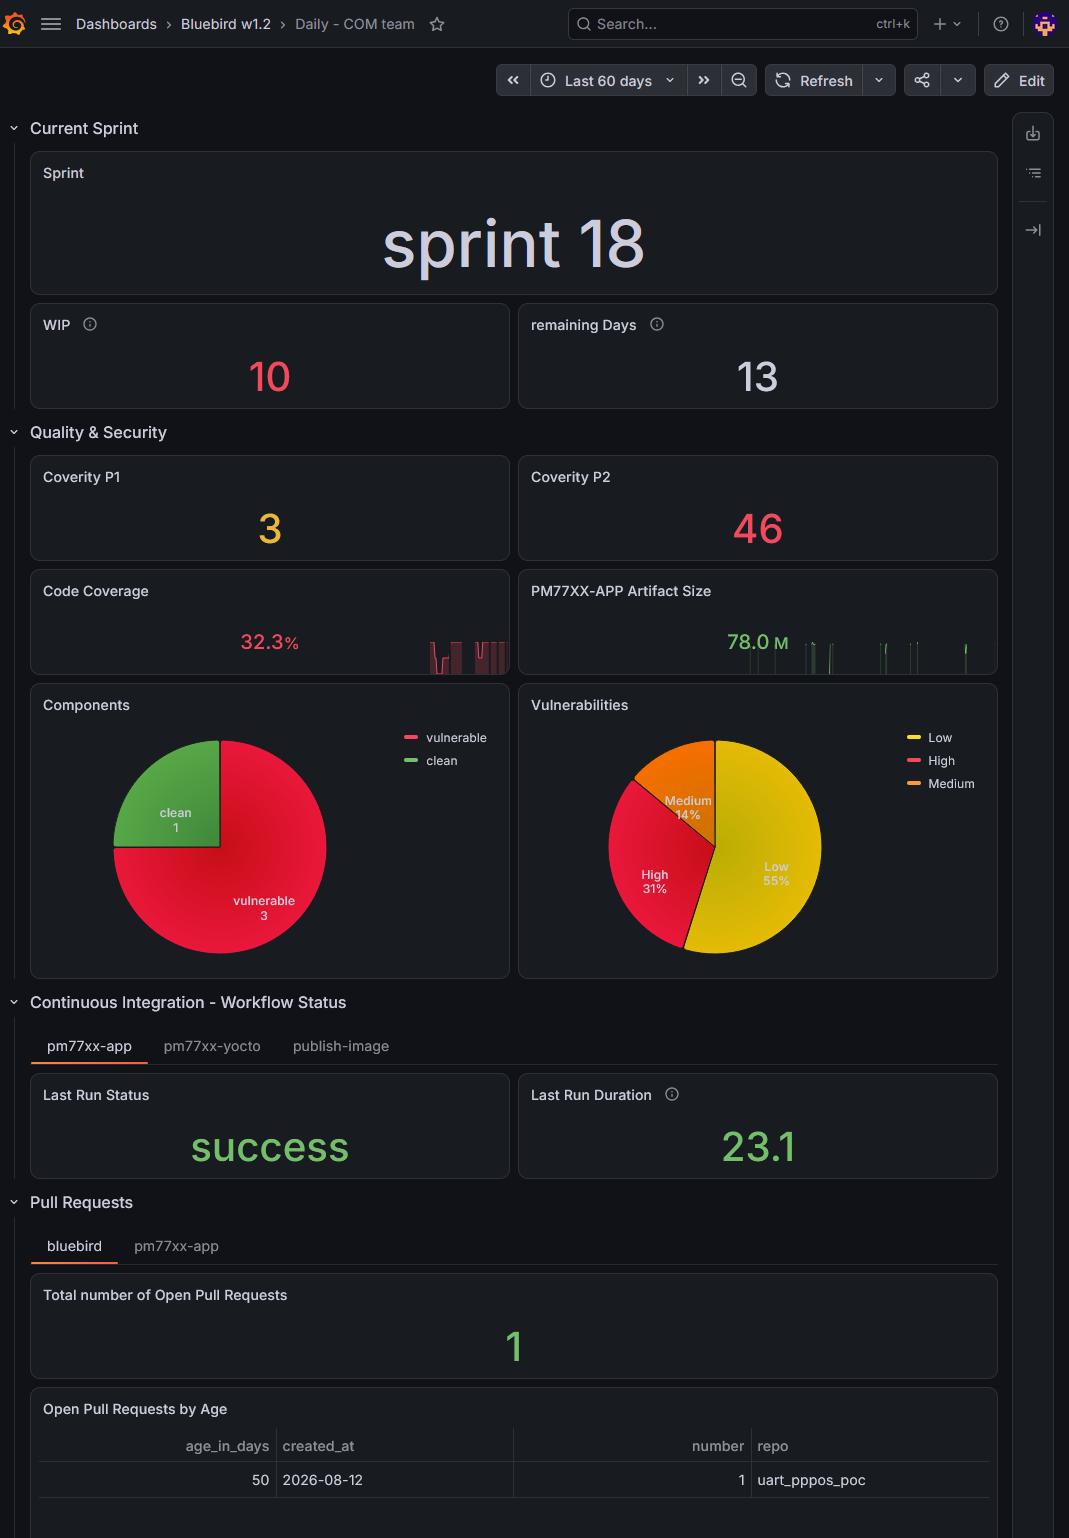
\includegraphics[width=0.6\textwidth]{dashboard-grafana}
\caption{Tableau de bord Grafana de l'équipe COM}
\label{fig:impl-grafana}
\end{figure}

% ===========================================================================
\subsection{Bilan}
\label{ssec:impl-bilan}

\subsubsection{Couverture des exigences}

Le tableau~\ref{tab:impl-bilan-ef} indique, pour chaque groupe d'exigences
fonctionnelles, la section qui les traite et leur état.

\begin{table}[H]
\centering
\caption{Couverture des exigences fonctionnelles}
\label{tab:impl-bilan-ef}
\small
\begin{tabularx}{\textwidth}{@{}l X l l@{}}
\toprule
\textbf{Réf.} & \textbf{Constat} & \textbf{Section} & \textbf{État} \\
\midrule
EF1, EF2 & Matrice native/croisée $\times$ DEBUG/RELEASE & \ref{sec:impl-pipeline-app} & Couverte \\
EF3 & Coverity en trois phases, rapports P1/P2 & \ref{ssec:impl-coverity} & Couverte \\
EF4 & Scan BDBA de l'archive RELEASE/aarch64 & \ref{ssec:impl-bdba} & Couverte \\
EF5, EF7, EF8 & Tests unitaires, couverture, synthèse & \ref{ssec:impl-ut} & Couverte \\
EF6 & Robot Framework, désactivé par défaut, DEBUG/amd64 & \ref{ssec:impl-robot} & Partielle \\
EF9 & Version fixe, pas d'empreinte de commit dans le nom & \ref{ssec:impl-publication-app} & Partielle \\
EF10 à EF13 & Cinq variantes, \gls{sdk}, publication & \ref{sec:impl-pipeline-yocto} & Couverte \\
EF14 à EF17 & Image versionnée, validée, publiée & \ref{sec:impl-conteneur} & Couverte \\
EF18, EF20, EF21 & Collecte, historisation, Grafana & \ref{ssec:impl-observabilite} & Couverte \\
EF19, EF22 & Deux formats d'import ; évolution des constructions limitée au dernier run & \ref{ssec:impl-observabilite} & Partielle \\
\bottomrule
\end{tabularx}
\end{table}

Pour les exigences non fonctionnelles, ENF1, ENF2, ENF4, ENF5, ENF8, ENF9,
ENF12 à ENF14 et ENF19 à ENF21 sont couvertes par les choix décrits plus haut.
ENF3 (traçabilité des artefacts) est partielle, pour la raison donnée pour
EF9. ENF6 (cache partagé de la distribution) n'est pas couverte : l'étude
NFS/snapshot a conduit à retenir la solution NFS. ENF11 (mutualisation entre les équipes COM et
MET) n'a pas été traitée.

\subsubsection{Difficultés transverses}

Le débogage des scripts bash et Python a occupé une part notable du travail.
Les problèmes récurrents étaient :

\begin{itemize}[nosep]
  \item un code de sortie significatif (\texttt{extract\_cov.sh}) interprété comme un
        échec par la plateforme ;
  \item des chemins qui varient selon l'image dans laquelle s'exécute le job
        (artefacts, répertoire de travail) ;
  \item des étapes qui ne terminent jamais, d'où les \texttt{timeout-minutes} ;
  \item des citations de secrets et de chaînes dans les scripts embarqués dans le YAML,
        déplacés dans \texttt{scripts/} pour être testables (principe P1).
\end{itemize}

Les limites qui découlent de ce bilan sont discutées en
section~\ref{sec:eval-discussion}, et les perspectives correspondantes en
section~\ref{sec:concl-perspectives}.


% ============================================================================
%  Chapitre 6 — Évaluation et résultats
%  Cible : 10 à 12 pages. À rédiger J10-J11.
%
%  AVERTISSEMENT : ce chapitre ne peut être rédigé qu'une fois les mesures
%  collectées (voir scripts/collecte-mesures.sh et annexe B).
%  Aucune valeur ne doit être inventée. Si une mesure « avant » n'est pas
%  disponible, l'écrire explicitement et en faire une limite méthodologique.
% ============================================================================
\chapter{Évaluation et résultats}
\label{chap:evaluation}

\section{Protocole d'évaluation}
\label{sec:eval-protocole}

\subsection{Questions d'évaluation}
L'évaluation vise à répondre aux quatre sous-questions posées en
section~\ref{sec:intro-problematique} :

\begin{description}[style=nextline,leftmargin=1.5cm]
  \item[QE1] L'environnement de construction obtenu est-il effectivement
    reproductible ?
  \item[QE2] L'intégration des analyses de sécurité améliore-t-elle la
    détection des défauts sans dégrader la vélocité ?
  \item[QE3] Les indicateurs collectés permettent-ils de piloter la qualité ?
  \item[QE4] L'infrastructure d'exécution est-elle maîtrisée en coût et en
    effort d'administration ?
\end{description}

\subsection{Sources de mesure}
\begin{table}[H]
\centering
\caption{Sources des mesures utilisées}
\label{tab:eval-sources}
\begin{tabularx}{\textwidth}{@{}l X l@{}}
\toprule
\textbf{Indicateur} & \textbf{Source} & \textbf{Période} \\
\midrule
Durée et issue des exécutions & Interface de la plateforme d'orchestration & \\
Couverture de code & Rapports de l'outil de couverture & \\
Défauts d'analyse statique & Vues du serveur d'analyse & \\
Vulnérabilités de composants & Rapports de l'analyseur binaire & \\
Effort d'administration & Relevé déclaratif auprès de l'équipe & \\
\bottomrule
\end{tabularx}
\end{table}

\aecrire{Préciser la période d'observation, le nombre d'exécutions prises en
compte, et le traitement des valeurs aberrantes (exécutions interrompues,
indisponibilité d'un service externe). Une évaluation sans protocole explicite
n'est pas défendable.}

\subsection{Validité}
\aecrire{Section courte mais indispensable. Traiter : validité interne (les
améliorations sont-elles attribuables à la chaîne ou à d'autres évolutions
concomitantes ?), validité externe (généralisation à d'autres produits),
fiabilité (les mesures sont-elles reproductibles ?).}

% ===========================================================================
\section{Impact}
\label{sec:eval-impact}

\aecrire{Section chapeau (2-3 phrases) : annoncer que cette section restitue
les effets de la chaîne au-delà de la seule mesure technique — indicateurs de
performance de livraison, coût, retour des équipes.}

\subsection{Indicateurs de performance de livraison}
\label{sec:eval-dora}

\begin{table}[H]
\centering
\caption{Indicateurs de performance adaptés au contexte embarqué}
\label{tab:eval-dora}
\begin{tabularx}{\textwidth}{@{}l X c c@{}}
\toprule
\textbf{Indicateur} & \textbf{Adaptation retenue} & \textbf{Avant} & \textbf{Après} \\
\midrule
Fréquence d'intégration & Nombre d'intégrations validées par semaine & & \\
Délai de retour & Délai entre soumission et résultat complet & & \\
Taux d'échec & Part des exécutions en échec imputables au code & & \\
Délai de rétablissement & Temps de remise en état d'une chaîne cassée & & \\
\bottomrule
\end{tabularx}
\end{table}

\aecrire{Justifier chaque adaptation par rapport à la définition d'origine
(section~\ref{sec:art-dora}). Si les valeurs « avant » sont estimées et non
mesurées, l'indiquer dans le tableau et dans le texte.}

\subsection{Coût et effort d'administration}
\label{sec:eval-cout}

\aecrire{Estimer : coût d'exécution de l'infrastructure, temps d'ingénierie
économisé sur les tâches auparavant manuelles (analyse de composants avant
jalon, préparation des environnements, collecte des rapports), et effort de
maintenance de la chaîne elle-même. Ne pas dissimuler ce dernier poste : une
chaîne d'intégration a un coût de possession.}

\subsection{Retour des utilisateurs}
\label{sec:eval-retour}

\aecrire{Si un recueil auprès des développeurs est possible dans les délais,
même informel, l'intégrer : quelques verbatims bien choisis renforcent
considérablement une étude de cas. Préciser le nombre de personnes
interrogées et la méthode.}

\subsection{Apports pour l'entreprise}
\label{sec:eval-apports-entreprise}

\aecrire{Distinguer l'apport technique de l'apport organisationnel : au-delà
de l'outillage, la chaîne modifie les pratiques de l'équipe, rend visible la
qualité et fournit les éléments de preuve attendus par le cadre normatif.}

% ===========================================================================
\section{Difficultés rencontrées}
\label{sec:eval-difficultes}

\aecrire{Section chapeau : consolider ici les difficultés concrètes
rencontrées pendant la mise en œuvre (renvoyer aux difficultés déjà détaillées
section~\ref{sec:impl-pipeline-app} pour la chaîne applicative) et celles
propres à la mesure elle-même.}

\subsection{Difficultés techniques}
\aecrire{Reprendre et synthétiser les difficultés déjà documentées au
chapitre~5 : nettoyage des services en fin d'exécution sur un exécuteur neuf,
délai d'attente au démarrage des services, exclusion des tests destinés au
cœur temps réel, normalisation des chemins pour l'analyse statique sur
exécuteurs jetables.}

\subsection{Difficultés liées à la mesure}
\aecrire{Distinguer des limites méthodologiques (traitées en section
Discussion) : il s'agit ici des obstacles concrets rencontrés pour collecter
les mesures elles-mêmes — étude de cas unique, mesures partiellement
déclaratives, effet d'apprentissage de l'équipe concomitant à la période
d'observation.}

% ===========================================================================
\section{Résultats}
\label{sec:eval-resultats}

\aecrire{Section chapeau (2-3 phrases) : annoncer que cette section présente
les résultats quantitatifs obtenus, dans l'ordre reproductibilité,
performance, puis qualité et sécurité.}

\subsection{Reproductibilité de l'environnement}
\label{sec:eval-reproductibilite}

\aecrire{Protocole proposé : construire une même révision du code à deux dates
distinctes et sur deux machines distinctes avec la même étiquette d'image,
puis comparer. Indiquer précisément ce qui est comparé : versions des outils,
réussite de la construction, et si possible empreinte des artefacts produits.
Discuter les écarts constatés et leurs causes (horodatages, chemins de
construction, ordre de liaison).}

\chiffre{Résultat de la comparaison des empreintes d'artefacts.}

\subsection{Performance de la chaîne}
\label{sec:eval-performance}

\subsubsection{Durées de construction}
\begin{table}[H]
\centering
\caption{Durées de construction observées}
\label{tab:eval-durees}
\begin{tabular}{@{}lccc@{}}
\toprule
\textbf{Chaîne} & \textbf{Minimum} & \textbf{Médiane} & \textbf{Maximum} \\
\midrule
Applicative (matrice complète) & & & \\
Distribution, variante dev & & & \\
Distribution, variante prod & & & \\
Publication de l'image de compilation & & & \\
\bottomrule
\end{tabular}
\end{table}

\subsubsection{Effet du cache d'état partagé}
\aecrire{Comparer construction à froid et à chaud. C'est un résultat
quantitatif fort et facile à obtenir : ne pas le négliger. Présenter sous
forme de tableau puis d'un graphique.}

\begin{figure}[H]
\centering
\aecrire{Graphique : durée de construction avec et sans cache, par variante.}
\caption{Incidence du cache d'état partagé sur la durée de construction}
\label{fig:eval-cache}
\end{figure}

\subsubsection{Effet du parallélisme de la matrice}
\aecrire{Comparer la durée cumulée des quatre configurations exécutées en
séquence à la durée réelle observée en parallèle.}

\subsection{Qualité et sécurité}
\label{sec:eval-qualite}

\subsubsection{Couverture de code}
\begin{figure}[H]
\centering
\aecrire{Graphique d'évolution de la couverture (lignes, fonctions, branches)
sur la période d'observation.}
\caption{Évolution de la couverture de code}
\label{fig:eval-couverture}
\end{figure}

\subsubsection{Défauts détectés par l'analyse statique}
\aecrire{Présenter la répartition initiale des défauts par priorité, puis leur
évolution. Distinguer les défauts préexistants des défauts nouvellement
introduits : c'est la distinction qui donne du sens à la mesure.}

\chiffre{Nombre de défauts de priorité 1 et 2 au démarrage et en fin de
période.}

\subsubsection{Vulnérabilités des composants tiers}
\aecrire{Présenter le nombre de composants identifiés et la répartition des
vulnérabilités par sévérité. Souligner l'apport principal : avant la mise en
place, l'inventaire des composants n'existait pas de manière automatisée.}

\subsubsection{Détection des régressions}
\aecrire{Si des cas concrets de régressions détectées par la chaîne avant
intégration sont documentés, les citer. Un exemple réel vaut mieux qu'un
paragraphe général.}

% ===========================================================================
\section{Discussion}
\label{sec:eval-discussion}

\subsection{Réponses aux questions d'évaluation}
\aecrire{Reprendre QE1 à QE4 et y répondre explicitement, en s'appuyant sur
les mesures présentées. Une réponse nuancée et argumentée est attendue.}


\subsection{Limites}
\aecrire{Recenser honnêtement : absence de tests sur cible matérielle réelle
dans la chaîne, politique de blocage non appliquée sur l'analyse statique,
exécution en superutilisateur, absence de mesure de référence antérieure pour
certains indicateurs, période d'observation courte. Une section de limites
solide est un marqueur de maturité, elle ne dessert pas la note.}

\subsection{Menaces à la validité}
\aecrire{Distinguer des limites : il s'agit ici de ce qui pourrait invalider
les conclusions. Étude de cas unique, mesures partiellement déclaratives,
effet d'apprentissage de l'équipe concomitant.}

% ============================================================================
%  Chapitre 7 — Conclusion et perspectives
%  Cible : 3 à 4 pages. À rédiger J12.
% ============================================================================
\chapter{Conclusion et perspectives}
\label{chap:conclusion}

\section{Rappel de la problématique et de la démarche}
\label{sec:concl-rappel}

\aecrire{Un paragraphe. Reformuler la question de recherche et résumer la
démarche suivie. Ne pas introduire d'élément nouveau.}

\section{Principaux résultats}
\label{sec:concl-resultats}

\aecrire{Reprendre les six contributions annoncées en
section~\ref{sec:intro-contributions} et, pour chacune, énoncer le résultat
obtenu en une à deux phrases, avec les valeurs chiffrées du chapitre~6. La
symétrie entre l'introduction et la conclusion est ce que le jury vérifie en
premier.}

\section{Apports pour l'entreprise}
\label{sec:concl-apports}

\aecrire{Distinguer l'apport technique de l'apport organisationnel : au-delà
de l'outillage, la chaîne modifie les pratiques de l'équipe, rend visible la
qualité et fournit les éléments de preuve attendus par le cadre normatif.}

\section{Apports personnels}
\label{sec:concl-apports-perso}

\aecrire{Une demi-page, factuelle et sans emphase : compétences acquises,
difficultés surmontées, posture d'ingénieur au sein d'une organisation
industrielle.}

\section{Perspectives}
\label{sec:concl-perspectives}

\aecrire{Formuler des perspectives précises et réalistes, issues des limites
du chapitre~6. Éviter les généralités.}

\subsection{Court terme}
\begin{itemize}[nosep]
  \item Application d'une politique de blocage sur les défauts d'analyse
        statique nouvellement introduits.
  \item Exécution de la chaîne à chaque proposition de modification et non
        uniquement selon une planification quotidienne.
  \item Suppression de l'exécution en superutilisateur dans le conteneur de
        compilation.
\end{itemize}

\subsection{Moyen terme}
\begin{itemize}[nosep]
  \item Intégration du banc de test matériel dans la chaîne, afin d'exécuter
        les tests sur cible réelle et non uniquement en compilation native.
  \item Génération et publication d'une nomenclature logicielle normalisée
        associée à chaque livrable.
  \item Signature et attestation de provenance des artefacts produits.
\end{itemize}

\subsection{Long terme}
\begin{itemize}[nosep]
  \item Extension de la chaîne aux autres produits de la gamme, par
        factorisation des workflows réutilisables.
  \item Automatisation de la constitution du dossier de preuves attendu par le
        cadre normatif.
\end{itemize}


% --------------------------------------------------------------- Bibliographie
\backmatter
\cleardoublepage
\phantomsection
\addcontentsline{toc}{chapter}{Bibliographie}
\printbibliography[title={Bibliographie}]

% --------------------------------------------------------------- Annexes
\appendix
% ============================================================================
%  Annexe B — Données de mesure
%  Tableaux bruts ayant servi au chapitre 6. Permet la vérifiabilité.
% ============================================================================
\chapter{Données de mesure}
\label{ann:donnees}

\section{Relevé des exécutions}
\label{ann:releve-executions}

\aecrire{Tableau des exécutions retenues : identifiant, date, chaîne, issue,
durée. Produit par \texttt{scripts/collecte-mesures.sh}. Si le volume est
important, n'en présenter qu'un échantillon représentatif et indiquer
l'effectif total.}

\begin{table}[H]
\centering
\caption{Extrait du relevé des exécutions}
\label{tab:ann-executions}
\begin{tabular}{@{}llllr@{}}
\toprule
\textbf{Id.} & \textbf{Date} & \textbf{Chaîne} & \textbf{Issue} & \textbf{Durée (min)} \\
\midrule
 & & & & \\
\bottomrule
\end{tabular}
\end{table}

\section{Mesures de couverture}
\label{ann:releve-couverture}

\aecrire{Relevé des taux de couverture lignes, fonctions et branches sur la
période d'observation.}

\section{Relevé des défauts d'analyse statique}
\label{ann:releve-defauts}

\aecrire{Nombre de défauts par priorité aux dates de relevé.}

\section{Relevé des vulnérabilités de composants}
\label{ann:releve-vulns}

\aecrire{Nombre de composants et répartition des vulnérabilités par sévérité.}

\section{Protocole de mesure de reproductibilité}
\label{ann:protocole-repro}

\aecrire{Décrire pas à pas la procédure appliquée en
section~\ref{sec:eval-reproductibilite}, de manière qu'un tiers puisse la
rejouer.}


\end{document}
